% AxiomForge manuscript — template version 1.0.0.
% Build: latexmk -pdf main.tex   (see README.md)
\documentclass[11pt]{amsart}
\makeatletter
% AxiomForge manuscript preamble — template version 1.0.0.
% This file is copied into every contribution and is owned by it afterwards.
% It fixes the typographic identity of the series; it defines no mathematical notation
% (each paper keeps its own notation in macros.tex).

% ---------------------------------------------------------------- page and fonts
\usepackage[a4paper,hmargin=31mm,top=34mm,bottom=36mm,headsep=10mm,footskip=12mm]{geometry}
\usepackage[T1]{fontenc}
\usepackage[utf8]{inputenc}
\usepackage{lmodern}
\usepackage{amsmath,amssymb,amsthm,mathtools}
\usepackage[final,protrusion=true,expansion=true]{microtype}
\usepackage{booktabs}
\usepackage{array}
\usepackage[shortlabels]{enumitem}
\setlist{itemsep=0.2em,topsep=0.4em}
\usepackage{xcolor}
\linespread{1.04}
\setlength{\emergencystretch}{1.5em}
\allowdisplaybreaks[1]
\numberwithin{equation}{section}
\setcounter{tocdepth}{2}
% Table of contents: sections (and their page numbers) in bold with a little space above
% them, subsections indented in normal weight; after \appendix only the (bold) section
% titles are listed, so the appendices never crowd the contents.
\def\l@section{\@tocline{1}{2.5pt plus 1pt minus 2pt}{0pt}{}{\bfseries\let\@tocpagenum\af@tocpagenumbf}}
\def\af@tocpagenumbf#1{\hss{\bfseries #1}}
\def\l@subsection{\@tocline{2}{0pt}{1.5em}{2.3em}{}}
\g@addto@macro\appendix{\addtocontents{toc}{\protect\setcounter{tocdepth}{1}}}
% Every appendix starts on a new page; the unnumbered back matter (\afbacksection) keeps the
% original \section and flows normally after the last appendix.
% (Local implementation through a hook, so that \section itself is not redefined.)
\newif\ifaf@appendixpage
\AddToHook{cmd/section/before}{\ifaf@appendixpage\clearpage\fi}
\g@addto@macro\appendix{\global\af@appendixpagetrue}

% ---------------------------------------------------------------- links
\definecolor{afblue}{rgb}{0.08,0.18,0.42}
\usepackage[pdfusetitle,bookmarks=true,bookmarksnumbered=true,bookmarksopen=true,
  colorlinks=true,linkcolor=afblue,citecolor=afblue,urlcolor=afblue,
  pdfpagelabels=true,pdfdisplaydoctitle=true]{hyperref}
\usepackage[capitalise,noabbrev]{cleveref}
% Local addition: unique PDF anchors for theorem-like environments numbered within sections.
\hypersetup{hypertexnames=false}

% ---------------------------------------------------------------- theorem environments
% thmtools keeps cleveref names correct for environments sharing one counter.
\usepackage{thmtools}
\declaretheorem[style=plain,numberwithin=section,name=Theorem]{theorem}
\declaretheorem[style=plain,sibling=theorem,name=Proposition]{proposition}
\declaretheorem[style=plain,sibling=theorem,name=Lemma]{lemma}
\declaretheorem[style=plain,sibling=theorem,name=Corollary]{corollary}
\declaretheorem[style=plain,numbered=no,name=Theorem]{theorem*}
\declaretheorem[style=definition,sibling=theorem,name=Definition]{definition}
\declaretheorem[style=definition,sibling=theorem,name=Example]{example}
\declaretheorem[style=remark,sibling=theorem,name=Remark]{remark}
\crefname{equation}{}{}
\Crefname{equation}{Equation}{Equations}

% ---------------------------------------------------------------- series metadata
% \afidentifier{AF-0001}, \afversion{1.0.0}, \afdate{25 November 2026},
% \afrepository{https://github.com/axiomforge-math/mathematics/tree/main/results/...},
% \afdisclosure{short AI-assisted research disclosure},
% \afstatus{verification status} (local addition; optional)
\newcommand{\afidentifier}[1]{\gdef\af@identifier{#1}}
\newcommand{\afversion}[1]{\gdef\af@version{#1}}
\newcommand{\afdate}[1]{\gdef\af@date{#1}}
\newcommand{\afrepository}[1]{\gdef\af@repository{#1}}
\newcommand{\afdisclosure}[1]{\gdef\af@disclosure{#1}}
\newcommand{\afcorrespondence}[1]{\gdef\af@correspondence{#1}}
\gdef\af@correspondence{}
% Local addition: verification status of the contribution, printed as a 'Status' row.
\newcommand{\afstatus}[1]{\gdef\af@status{#1}}
\gdef\af@status{}

% The publication block printed under the abstract on the title page.
\newcommand{\afpublicationblock}{%
  \begingroup\footnotesize\noindent
  \begin{tabular}{@{}l@{\quad}p{0.72\textwidth}@{}}
    \textit{Identifier} & \af@identifier\quad(version \af@version, \af@date)\\[1pt]
    \ifx\af@status\@empty\else\textit{Status} & \af@status\\[1pt]\fi
    \textit{Repository} & \url{\af@repository}\\[1pt]
    \ifx\af@correspondence\@empty\else\textit{Correspondence} & \af@correspondence\\[1pt]\fi
    \textit{Disclosure} & \af@disclosure
  \end{tabular}\par
  \endgroup}

% Front matter: title page, then contents, then the body on a fresh page.
\newcommand{\affrontmatter}{%
  \maketitle
  \vspace*{\fill}
  \afpublicationblock
  \thispagestyle{plain}%
  \clearpage
  {\hypersetup{linkcolor=black}\fontsize{9}{10.6}\selectfont\tableofcontents}
  \clearpage}

% Unnumbered back-matter sections (amsart lists starred sections in the contents).
\newcommand{\afbacksection}[1]{\global\af@appendixpagefalse\section*{#1}}

% ---------------------------------------------------------------- local to this paper
% (contour figure and line breaks in long URLs)
\hbadness=10000 % no underfull-box reports: the log of the bibliography contains a T1 accented letter, which the archive tool cannot decode
\usepackage{tikz}
\usetikzlibrary{decorations.pathreplacing}
\g@addto@macro\UrlBreaks{\do\-}

\makeatother
% Notation local to this paper. Define only what materially simplifies the exposition.
\newcommand{\N}{\mathbb{N}}
\newcommand{\Z}{\mathbb{Z}}
\newcommand{\Q}{\mathbb{Q}}
\newcommand{\R}{\mathbb{R}}
\newcommand{\C}{\mathbb{C}}
\newcommand{\Fp}{\mathbb{F}_p}
\newcommand{\Zp}{\mathbb{Z}_{(p)}}

\DeclareMathOperator{\den}{den}
\DeclareMathOperator{\rank}{rank}
\DeclareMathOperator{\Res}{Res}
\DeclareMathOperator{\adj}{adj}

\newcommand{\abs}[1]{\lvert #1\rvert}
\newcommand{\dd}{\mathrm{d}}
\newcommand{\e}{\mathrm{e}}

% The numbers, the function and its rational data.
\newcommand{\trig}{\psi_1}
\newcommand{\alt}{\mathrm{alt}}
\newcommand{\sep}{\mathrm{sep}}

% The letter k in the title (a macro, so that amsart's upper-casing leaves it alone).
\newcommand{\titlek}{k}

% Node sets.
\newcommand{\Com}{\mathcal{C}}   % common nodes
\newcommand{\Nod}{\mathcal{Z}}   % all nodes
\newcommand{\Bor}{\mathcal{B}}   % border nodes
\newcommand{\Row}{\mathcal{R}}   % row nodes
\newcommand{\Col}{\mathcal{Q}}   % column nodes

% Constants of the comparison.
\newcommand{\cA}{\mathsf{A}}     % arithmetic constant
\newcommand{\cD}{\mathsf{D}}     % decay constant

% Logarithmic potential theory.
\newcommand{\pot}[1]{U^{#1}}
\newcommand{\Atoms}{\mathcal{P}}

% File paths, programs and Lean identifiers (breakable).
\newcommand{\file}[1]{\nolinkurl{#1}}
\newcommand{\TRENDEXTRA}{}%TEMP


\title[Trigamma differences at fifths and one half: a candidate proof]{The irrationality of
  $\psi_1(k/5)-\pi^2/2$: a candidate proof with separated L\"owner determinants}
\author{AxiomForge}
\urladdr{https://github.com/axiomforge-math}
\subjclass[2020]{Primary 11J72; Secondary 33B15, 31A15}
\keywords{Irrationality, trigamma function, L\"owner determinants, divided differences,
  logarithmic potential theory, computer-assisted proof}
\date{26 November 2026}

\afidentifier{AF-0002}
\afversion{0.1.0}
\afdate{26 November 2026}
\afstatus{Preprint. Candidate proof: complete on paper, not yet independently verified; no human
  review. It rests on two computer-assisted certificates, recomputed in an AI-internal audit,
  whose comparison leaves a certified margin of only $0.000754$ per $h^2$ (\cref{tab:status}).}
\afrepository{https://github.com/axiomforge-math/mathematics/tree/main/results/AF-0002-trigamma-fifths-irrationality}
\afcorrespondence{\href{mailto:axiomforge.math@gmail.com}{axiomforge.math@gmail.com}}
\afdisclosure{AI-assisted research. The original exploration and candidate proof were
  produced by GPT-6.2 XHigh (web version); the reconstruction, audits, this manuscript and the Lean
  formalization by Claude Opus~5.5 (Anthropic), and an adversarial review and the resulting revision
  by Claude Fable~5.2 (Anthropic), under the direction of AxiomForge. No AI review is independent, and
  no human review has taken place. Details in the AI-assisted research disclosure at the end.}

\begin{document}

\begin{abstract}
For $k=1,2,3,4$ we give a candidate proof that $\xi_k=\trig(k/5)-\pi^2/2$ is irrational,
where $\trig$ is the trigamma function; since $\trig(1/2)=\pi^2/2$, the number $\xi_k$ is the
difference $\trig(k/5)-\trig(1/2)$. The statement concerns neither $\trig(k/5)$ itself nor
$\trig(k/5)-\pi^2/6$. The proof studies determinants of L\"owner (divided-difference)
matrices of $\psi(z+k/5)-\psi(z+1/2)$ on $h$ common nodes and $h/8$ border nodes, in the
framework of S.~Litsey, who lists these numbers among those that his interleaved (alternating)
border does not reach. The new ingredient is to separate the border rows from the border
columns. An Andr\'eief--Cauchy factorization shows that this divides every determinant by
exactly $2^{m(m-1)}$, $m=h/16$, without changing any odd-prime valuation, while an entrywise bound
controls the prime $2$ at cost $O(h\log h)$; the net gain is $(\log 2)/256$ per $h^2$. With a
two-layer $p$-adic bound for the denominators, integrated over primes in progressions
modulo~$5$, and a logarithmic-energy bound for the size, we obtain
$\log\den\le(3.5121304+o(1))h^2$ and $\log\abs{\det}\le-(3.5128848+o(1))h^2$. The
margin, $0.000754$ per $h^2$, is thin and rests on two computer-assisted certificates, in exact
rational and in ball arithmetic. Both were recomputed, by implementations written separately
from the original programs, in an internal audit performed by an AI system; the separation
identity was examined in a second AI-internal review. No numerical experiment at accessible sizes
can test the final inequality, no AI review is independent, and no human has reviewed the
argument: the result is a candidate.
\end{abstract}

\affrontmatter

\section{Introduction}\label{sec:introduction}

\subsection{The result}\label{subsec:result}

Let $\psi=\Gamma'/\Gamma$ be the digamma function and $\trig=\psi'$ the trigamma function, so
that $\trig(x)=\sum_{j\ge0}(j+x)^{-2}$ for $x>0$. Since $\trig(1/2)=\pi^2/2$
\cite[5.15.3]{DLMF}, the numbers
\begin{equation}\label{eq:xi-def}
  \xi_k:=\trig\!\left(\tfrac k5\right)-\frac{\pi^2}{2}
       =\trig\!\left(\tfrac k5\right)-\trig\!\left(\tfrac12\right),\qquad k=1,2,3,4,
\end{equation}
are differences of trigamma values at a fifth and at one half. Equivalently
$\xi_k=\sum_{n\ge1}a_k(n)n^{-2}$ with $a_k(n)=25\cdot\mathbf 1[n\equiv k\bmod 5]-3$. Numerically
$\xi_1=21.3325750\ldots$, $\xi_2=2.3405543\ldots$, $\xi_3=-1.2985925\ldots$ and
$\xi_4=-2.6353280\ldots$.

\begin{theorem}\label{thm:main}
For each $k\in\{1,2,3,4\}$ the number $\xi_k=\trig(k/5)-\pi^2/2$ is irrational.
\end{theorem}

\Cref{thm:main} is a \emph{candidate} result. Its proof is complete on paper and rests on two
computer-assisted certificates, but several steps have not yet been independently verified and
no human referee has checked the argument; \cref{subsec:status} records the status of each step.
The final comparison has a certified margin of $0.000754$ per $h^2$ between quantities of size
about $3.5$ per $h^2$, so a relative error of order $10^{-4}$ in either certificate could
invalidate the proof.

\Cref{thm:main} says nothing about $\trig(k/5)$ itself, nor about the numbers
$\trig(k/5)-\pi^2/6=\trig(k/5)-\trig(1)$, for which Litsey states an irrationality measure
\cite[Theorem~1.6(ii)]{Litsey2026Lowner}. The latter differ from $\xi_k$ by $\pi^2/3$, and since
the linear independence of $1$, $\pi^2$ and $\trig(k/5)$ over $\Q$ is not known, neither statement
implies the other. We prove no irrationality measure.

\subsection{The argument in outline}\label{subsec:one-page}

Fix $k$, put $s=k/5$ and $F(z)=\psi(z+s)-\psi(z+\frac12)$, so that $\xi_k=F'(0)$; for integers
$x\ge0$ the numbers $f_x=F(x)-F(0)$ and $d_x=F'(x)-F'(0)$ are explicit rationals. Let
$h\in16\N$ and $m=h/16$. All rates below are per $h^2$, as $h\to\infty$ through $16\N$, and
$\den r$ is the denominator of a rational number $r$. The nodes are $0,1,\dots,h+2m-1$. We call $0,\dots,h-1$ the
\emph{common nodes}: they serve as rows and as columns. We call $h,\dots,h+2m-1$ the
\emph{border}: $m$ of these nodes serve as rows and $m$ as columns. In what we call the \emph{alternating} geometry the border rows are
$h,h+2,h+4,\dots$; in what we call the \emph{separated} geometry they are $h,\dots,h+m-1$. A
set $I$ of at most one common node removed from rows and columns is called a \emph{deletion}.
The pencil $P^\star_I(X)\in\Q[X]$, $\star\in\{\alt,\sep\}$, is the determinant of the matrix with
entries $(f_y-f_x)/(y-x)$ for a row node $x$ and a column node $y\ne x$, and $X+d_x$ at the
common diagonal positions. At $X=\xi_k$ it is the L\"owner determinant
$\det\bigl[(F(y)-F(x))/(y-x)\bigr]$, the diagonal entries being $F'(x)$. The border has $2m=h/8$
nodes; this ratio $c=\frac18$ has no other justification than that the two certificates were
computed for it (\cref{rem:separation-meaning}).

\emph{The criterion.} If $\xi_k$ were rational and $P^{\sep}_{I_h}(\xi_k)\ne0$, then
$\den\bigl(P^{\sep}_{I_h}(\xi_k)\bigr)\cdot\abs{P^{\sep}_{I_h}(\xi_k)}$ would be a positive integer,
hence at least $1$. It therefore suffices to prove three estimates, uniform in deletions
$\abs I\le1$, whose constants contradict this for large $h$.

\begin{table}[ht]
\centering
\small
\begin{tabular}{@{}>{\raggedright\arraybackslash}p{0.40\textwidth}>{\raggedright\arraybackslash}p{0.25\textwidth}>{\raggedright\arraybackslash}p{0.23\textwidth}@{}}
\toprule
estimate & certified constant & where\\
\midrule
(N) some $P^{\sep}_{I}(X)\ne0$, $\abs I\le1$, for every $X\in\C$ & exact, no constant & \cref{prop:nonvanishing}\\
(A) $\log\den P^{\sep}_I(X)\le(\cA+o(1))h^2$, $X\in\Q$ & $\cA=3.5121303755\ldots<3.5121304$ & \cref{thm:arithmetic}, \cref{prop:A-value}\\
(D) $\log\abs{P^{\sep}_I(\xi_k)}\le-(\cD_{\sep}+o(1))h^2$ & $\cD_{\sep}\ge3.5128848$ & \cref{cor:decay-separated}, \cref{prop:energy-certificate}\\
margin & $\cD_{\sep}-\cA\ge3.5128848-3.5121304\ge0.000754$ & \cref{subsec:main-proof}\\
\bottomrule
\end{tabular}
\caption{The three estimates and the certified constants (per $h^2$). Here $\cA$ is an exact
rational number and an upper bound for the denominator rate, and $\cD_{\sep}$ is a certified lower
bound for the decay rate (a truncated decimal); neither is claimed to be the true rate.}
\label{tab:constants}
\end{table}

\emph{How the estimates are obtained.}
\begin{enumerate}[(1)]
  \item \emph{Separation} (\cref{sec:lowner}). By Andr\'eief's identity and Cauchy's double
  alternant, a L\"owner determinant depends on how its nodes are split into rows and columns only
  through the product $\Delta(\text{rows})\Delta(\text{columns})$ of the two Vandermonde products.
  Replacing two border progressions of step $2$ by two of step $1$ gives
  $P^{\sep}_I=2^{-m(m-1)}P^{\alt}_I$ in $\Q[X]$.
  \item \emph{Nonvanishing} (\cref{sec:nonvanishing}). Kernel vectors of the pencil correspond to
  pairs of interpolating polynomials. A discrete Wronskian, together with the absence of a
  rational solution of $r(z+1)-r(z)=F(z+1)-F(z)$, shows that the corank is at most one and that
  some diagonal cofactor is nonzero, which gives~(N).
  \item \emph{Small primes and $p=2$} (\cref{subsec:entry-bounds}). Entrywise bounds cost
  $o(h^2)$ at the primes $p\le\sqrt{5N}$, $N=h+2m$. At $p=2$ the bound is applied to the
  \emph{separated} matrix itself and costs only $O(h\log h)$; this is what protects the gain
  of~(1), since for the alternating determinant the factor $2^{m(m-1)}$ would have to be given
  back. By~(1), the odd-prime valuations of the two geometries coincide.
  \item \emph{Primes $p\asymp h$} (\cref{subsec:polar,subsec:nullspace,subsec:profile,subsec:integration}).
  Modulo $p^2$, the matrix $p^2M^{\alt}_I(X)$, where $M^{\alt}_I(X)$ is the pencil matrix, is
  block diagonal along residue classes of nodes modulo $p$, up to a term of order $p$ that
  vanishes inside the blocks. A Schur complement then bounds the exponent of $p$ in the
  denominator by twice the sum of the ranks of the blocks plus the rank of a pairing between
  their null vectors; all these are ranks of finitely many rational matrices. This yields a piecewise
  affine function of $p/h$, which we call the \emph{profile}, and the prime number theorem in
  progressions modulo $5$ integrates it to $\cA$ (computed exactly, \cref{sec:arith-certificate}).
  \item \emph{Size} (\cref{sec:decay}). The reflection formula moves the L\"owner integrals to a
  contour in $\operatorname{Re}z<0$ on which the density decays like $\e^{-2\pi\abs{\operatorname{Im}z}}$.
  Andr\'eief's identity turns $\abs{P^{\alt}_I(\xi_k)}$ into a multiple integral whose logarithm
  is a discrete logarithmic energy. Comparing with a trial measure by the positivity of the
  logarithmic energy gives $\cD_{\alt}\ge3.5101772$, certified in ball arithmetic
  (\cref{sec:contour-and-measure,sec:exact-formulas,sec:error-analysis}). By~(1),
  $\cD_{\sep}=\cD_{\alt}+(\log2)/256\ge3.5128848$.
  \item \emph{Conclusion} (\cref{sec:proof}). Since $\cA<\cD_{\sep}$, the positive integers of the
  criterion would tend to $0$, a contradiction.
\end{enumerate}
With these certificates alone, the comparison for the alternating geometry does not close: the
certified lower bound $\cD_{\alt}$ for the decay is smaller than the upper bound $\cA$ for the
denominators, by $0.00195$. This is a statement about our two bounds, not about the true rates;
we do not prove that the alternating border fails.

\subsection{Context and the new ingredient}\label{subsec:context}

Irrationality proofs for values of $\trig$ at rational points are rare. The value
$\trig(1)=\zeta(2)$ is the classical case (Ap\'ery; see~\cite{vanderPoorten1979,Beukers1979}),
and $\trig(1/2)=3\zeta(2)$ reduces to it. Calegari, Dimitrov and Tang~\cite{CDT2024} proved that
$1$, $\zeta(2)$ and $L(2,\chi_{-3})$ are linearly independent over $\Q$. This implies the
irrationality of $\trig(n/6)$ for every integer $n\ge1$, by the recurrence
$\trig(x+1)=\trig(x)-x^{-2}$ and the evaluations $\trig(\frac13)=4\zeta(2)+\frac92L(2,\chi_{-3})$,
$\trig(\frac16)=12\zeta(2)+\frac{45}2L(2,\chi_{-3})$ and their reflections. For the modulus $5$ the
only earlier statement about an individual number $\trig(k/5)+r\pi^2$, $r\in\Q$, that we know of is
Litsey's irrationality measure for $r=-\frac16$ \cite[Theorem~1.6(ii)]{Litsey2026Lowner}. We know
of no earlier proof of irrationality for $r=-\frac12$, the case treated here; our search of the
literature was made by an AI system, covered the sources listed in the disclosure at the end, and
is not a proof of absence. The results
on many irrational values of Dirichlet $L$-functions (see~\cite{Fischler2020L,RivoalZudilin2003}
and the survey~\cite{Fischler2004Bourbaki}) do not decide individual values of weight two. The
reflection formula $\trig(x)+\trig(1-x)=\pi^2/\sin^2(\pi x)$ \cite[5.15.6]{DLMF} gives the weaker
statement that at least one number in each pair $\{\xi_k,\xi_{5-k}\}$ is irrational, since
\begin{equation}\label{eq:pair-sum}
  \xi_k+\xi_{5-k}=\pi^2\cot^2\!\left(\tfrac{\pi k}5\right),\qquad
  \cot^2\!\left(\tfrac\pi5\right)=1+\tfrac2{\sqrt5},\quad
  \cot^2\!\left(\tfrac{2\pi}5\right)=1-\tfrac2{\sqrt5},
\end{equation}
is transcendental (\cref{rem:pairwise}).

Our method is the determinantal approach to irrationality~\cite{Zudilin2017} in the form
developed by Litsey~\cite{Litsey2026Lowner}, who uses L\"owner determinants with an alternating
border and, according to \cite[\S1.2]{Litsey2026Lowner}, takes the underlying framework from the
proof of the irrationality of Catalan's constant in~\cite{OpenAICatalan2026}. The numbers $\xi_k$
appear in \cite[\S12.1]{Litsey2026Lowner} among the constants that the alternating border does
not reach. That section consists of numerical observations outside the proofs of the paper; for
the border ratio $2m/h=\frac18$ it reports an estimated deficit of about $0.0014$ per $h^2$, with
a stated numerical error of about $2\cdot10^{-4}$, and of about $0.001$ if the local bounds and
the decay estimate were sharp. We quote these figures as reported there (version~3); we have not
reproduced them, and nothing below depends on them. Our own certified bounds for the alternating
geometry differ by $0.00195$ (\cref{subsec:margin}), which is an upper bound for the deficit of our
estimates and not a measurement of the true one. Both
works~\cite{Litsey2026Lowner,OpenAICatalan2026} are unrefereed and largely AI-generated; we use
them for orientation and attribution only, and the arguments below are self-contained apart from
standard facts, which we cite.

The new ingredient is to separate the border rows from the border columns
(\cref{fig:geometries}). This changes the determinant by the exact factor $2^{-m(m-1)}$ and
leaves every odd-prime valuation unchanged. The entrywise bound at $p=2$
(\cref{lem:entry-bound}), applied to the alternating determinant, gives no information about its
divisibility by $2^{m(m-1)}$. In the
separated geometry the same power of $2$ is gained in absolute value, while the denominator at
$p=2$ costs only $O(h\log h)$. The gain $m(m-1)\log2=(\frac{\log2}{256}+o(1))h^2$, with
$(\log2)/256=0.0027076\ldots$, exceeds the difference $0.00195$ between our two certified bounds
for the alternating geometry by $0.000754$.

\begin{figure}[ht]
\centering
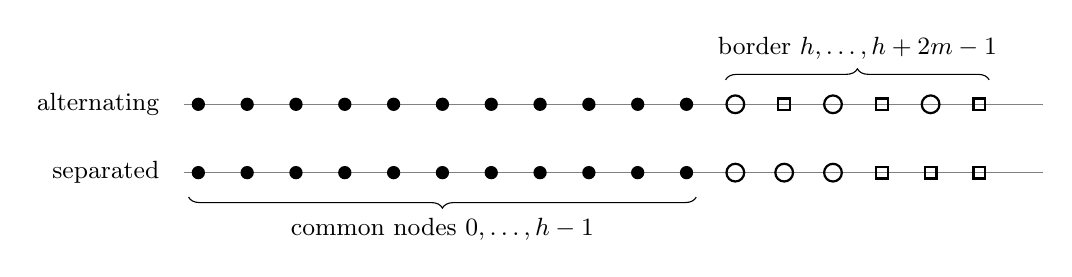
\begin{tikzpicture}[x=0.62cm,y=0.62cm]
  \foreach \yy/\lab in {1.4/alternating, 0/separated}{
    \node[anchor=east] at (-0.6,\yy) {\small\lab};
    \draw[gray] (-0.3,\yy) -- (17.3,\yy);
    \foreach \x in {0,...,10} {\fill (\x,\yy) circle (2.4pt);}
  }
  \foreach \x in {11,13,15}{\draw[thick] (\x,1.4) circle (3.2pt);}
  \foreach \x in {12,14,16}{\draw[thick] (\x-0.12,1.28) rectangle (\x+0.12,1.52);}
  \foreach \x in {11,12,13}{\draw[thick] (\x,0) circle (3.2pt);}
  \foreach \x in {14,15,16}{\draw[thick] (\x-0.12,-0.12) rectangle (\x+0.12,0.12);}
  \draw[decorate,decoration={brace,amplitude=4pt,mirror}] (-0.2,-0.5) -- (10.2,-0.5)
    node[midway,below=4pt] {\small common nodes $0,\dots,h-1$};
  \draw[decorate,decoration={brace,amplitude=4pt}] (10.8,1.9) -- (16.2,1.9)
    node[midway,above=4pt] {\small border $h,\dots,h+2m-1$};
\end{tikzpicture}
\caption{Schematic node geometries ($m=3$). Filled discs are common nodes, circles border rows,
squares border columns.}
\label{fig:geometries}
\end{figure}

\subsection{Status of the steps}\label{subsec:status}

\Cref{tab:status} gives the status of each step. \emph{Proved} means a complete proof, possibly
reviewed by an AI system; \emph{certified (AI-internal)} means a rigorous computation that was
recomputed, by implementations written separately from the original programs, in an internal
audit performed by an AI system (the \emph{AI-internal audit}); \emph{candidate} means a written
proof that has not been independently verified. A certified computation is only as good as the
statements that reduce the mathematics to it; these are listed in the table as separate steps.
No step has been checked by a human, and no AI review is independent certification. The open
points are listed in \cref{subsec:open-points}.

\begin{table}[ht]
\centering
\small
\begin{tabular}{@{}>{\raggedright\arraybackslash}p{0.34\textwidth}>{\raggedright\arraybackslash}p{0.20\textwidth}>{\raggedright\arraybackslash}p{0.36\textwidth}@{}}
\toprule
step & status & evidence\\
\midrule
separation identity (\cref{cor:separation}) & proved & AI-internal adversarial review; exact checks for $h\le64$\\
nonvanishing (\cref{prop:nonvanishing}) & candidate & no review; no rational roots for $h\le48$\\
entrywise bounds (\cref{lem:entry-bound}) & proved & elementary\\
polar congruences, nullspace bound (\cref{lem:two-layer}, \cref{prop:nullspace}) & candidate & checked in the AI-internal audit; finite tests up to $h=128$\\
profile bound and profile structure (\cref{lem:profile-bound}, \cref{lem:profile-structure}) & candidate & proofs written here, no review; affinity checked at five points of each cell\\
value of $\cA$ (\cref{prop:A-value}) & certified (AI-internal), given \cref{lem:profile-structure} & two exact implementations agree; the exact integration uses the breakpoints of \cref{lem:profile-structure}\\
prime number theorem bookkeeping (\cref{thm:arithmetic}) & candidate & standard; no review\\
contour representation, energy criterion (\cref{lem:contour}, \cref{prop:energy-criterion}) & candidate & inequality checked in the AI-internal audit\\
energy constants (\cref{prop:energy-certificate}) & certified (AI-internal) & ball arithmetic; the original fixed-point verifier gives a slightly weaker bound\\
final deduction (\cref{subsec:main-proof}) & proved & elementary; formalized in Lean conditionally on the estimates\\
\midrule
\cref{thm:main} & candidate & no human review\\
\bottomrule
\end{tabular}
\caption{Status of the steps of the proof.}
\label{tab:status}
\end{table}

\subsection{Notation and conventions}\label{subsec:notation}

Throughout, $k\in\{1,2,3,4\}$ and $s=k/5$; all logarithms are natural; implied constants in
$O(\cdot)$ and $o(\cdot)$ may depend on $k$ and on the rational number $X$ under consideration,
never on $h$, on a prime $p$ or on the deletion $I$; and asymptotic statements are as
$h\to\infty$ through $16\N$. \Cref{tab:notation} lists the notation used in more than one section.

\begin{table}[ht]
\centering
\small
\begin{tabular}{@{}>{\raggedright\arraybackslash}p{0.20\textwidth}>{\raggedright\arraybackslash}p{0.50\textwidth}>{\raggedright\arraybackslash}p{0.16\textwidth}@{}}
\toprule
symbol & meaning & defined in\\
\midrule
$F$, $\delta$ & $\psi(z+s)-\psi(z+\frac12)$, and $\delta(z)=F(z+1)-F(z)$ & \cref{subsec:function}\\
$f_x$, $d_x$ & $F(x)-F(0)$, $F'(x)-F'(0)$ for $x\in\Z_{\ge0}$ (rational) & \cref{subsec:function}\\
$h,m,n,N$ & $h\in16\N$, $m=h/16$, $n=h+m$, $N=h+2m$ & \cref{def:geometries}\\
$c$, $\lambda$ & border ratio $2m/h=\frac18$; $\lambda=n/h=\frac{17}{16}$ & \cref{def:geometries}\\
$\Nod,\Com,\Bor$ & all nodes $\{0,\dots,N-1\}$, common nodes $\{0,\dots,h-1\}$, border & \cref{def:geometries}\\
$\Row^\star,\Col^\star$ & row and column nodes, $\star\in\{\alt,\sep\}$ & \cref{def:geometries}\\
$I$, $n_I$ & deletion ($I\subseteq\Com$), size $n-\abs I$ of the pencil & \cref{def:geometries}\\
$M^\star_I(X)$, $P^\star_I(X)$ & L\"owner pencil and its determinant & \cref{def:pencil}\\
$g[x,y]$, $L_g(\Row,\Col)$ & divided differences of $g$, L\"owner matrix & \cref{subsec:partition}\\
$\Delta(S)$, $\omega_S$ & $\prod_{a<b}(x_b-x_a)>0$ and $\prod_{x\in S}(z-x)$ for $S=\{x_1<\dots<x_n\}\subset\R$; $\Delta(z)=\prod_{a<b}(z_b-z_a)$ for $z\in\C^n$ & \cref{subsec:andreief}\\
$\den r$, $v_p$, $e_p$, $\Zp$ & denominator of $r\in\Q$ ($\den0=1$), $p$-adic valuation, $e_p(r)=\max(0,-v_p(r))$, rationals with denominator prime to $p$ & \cref{sec:arithmetic}\\
$\kappa$, $V^\varepsilon_l$, $W^\varepsilon_l$ & root class of $p$ and polar values & \cref{subsec:polar}\\
$u$, $\gamma(t)$, $T(t)$ & the ratio $p/h$; numbers of common digits and of all digits of a fibre & \cref{subsec:profile}\\
$e_\kappa$, $\cA$ & profile and arithmetic constant & \cref{subsec:profile,subsec:integration}\\
$\nu$, $\mu$, $\Gamma$ & node measure, trial measure, contour & \cref{sec:decay}\\
$\pot\mu$, $I(\mu)$ & logarithmic potential and energy & \cref{subsec:energy-prelim}\\
$\cD_{\alt}$, $\cD_{\sep}$, $\cD^{*}_{\alt}$ & certified lower bounds for the decay rates of the two geometries (truncated decimals), and the certified rational bound & \cref{sec:decay}\\
\bottomrule
\end{tabular}
\caption{Notation.}
\small
\label{tab:notation}
\end{table}

\section{L\"owner pencils, the partition identity and separated borders}\label{sec:lowner}

This section defines the L\"owner pencils $P^\star_I(X)$ and proves the separation identity
$P^{\sep}_I=2^{-m(m-1)}P^{\alt}_I$ (\cref{cor:separation}). The identity is what makes the
argument work: it gives the factor $2^{-m(m-1)}$ in the size estimate of \cref{sec:decay} and
makes the odd-prime valuations of the two geometries equal, which is used throughout
\cref{sec:arithmetic}. Its proof rests on one observation (\cref{prop:partition}): a L\"owner
determinant depends on the split of its nodes into rows and columns only through the product of
the two Vandermonde products.

\subsection{The function and its rational data}\label{subsec:function}

Put
\[
  F(z)=\psi(z+s)-\psi\!\left(z+\tfrac12\right),\qquad s=\tfrac k5 .
\]
It is meromorphic in $\C$, with simple poles at $-s-a$ (residue $-1$) and at $-\tfrac12-a$
(residue $+1$), $a\in\Z_{\ge0}$, and $\xi_k=F'(0)$ by~\eqref{eq:xi-def}. Let
\[
  \delta(z)=\frac1{z+s}-\frac1{z+\frac12}.
\]
The recurrence $\psi(z+1)=\psi(z)+1/z$ \cite[5.5.2]{DLMF} gives $F(z+1)-F(z)=\delta(z)$ and
$F'(z+1)-F'(z)=\delta'(z)$; hence, for $x\in\Z_{\ge0}$,
\[
  f_x:=F(x)-F(0)=\sum_{j=0}^{x-1}\delta(j),\qquad
  d_x:=F'(x)-F'(0)=\sum_{j=0}^{x-1}\delta'(j)
\]
are rational numbers, explicitly
$f_x=\sum_{j<x}\bigl(\frac5{5j+k}-\frac2{2j+1}\bigr)$ and
$d_x=\sum_{j<x}\bigl(-\frac{25}{(5j+k)^2}+\frac4{(2j+1)^2}\bigr)$. In particular
\begin{equation}\label{eq:fd-increments}
  f_{x+1}-f_x=\delta(x),\qquad d_{x+1}-d_x=\delta'(x)\qquad(x\in\Z_{\ge0}).
\end{equation}

\subsection{Node sets and pencils}\label{subsec:pencils}

\begin{definition}[Geometries]\label{def:geometries}
Let $h\in16\N$ and put
\[
  m=\tfrac h{16},\qquad n=h+m,\qquad N=h+2m,\qquad c=\tfrac{2m}h=\tfrac18,\qquad
  \lambda=\tfrac nh=\tfrac{17}{16}.
\]
The nodes are $\Nod=\{0,1,\dots,N-1\}$, the common nodes
$\Com=\{0,\dots,h-1\}$ and the border $\Bor=\Nod\setminus\Com$. The alternating and separated
geometries are the pairs $(\Row^\star,\Col^\star)$ of row and column node sets
\begin{align*}
  \Row^{\alt}&=\Com\cup\{h+2r:0\le r<m\}, & \Col^{\alt}&=\Com\cup\{h+2r+1:0\le r<m\},\\
  \Row^{\sep}&=\Com\cup\{h+r:0\le r<m\}, & \Col^{\sep}&=\Com\cup\{h+m+r:0\le r<m\}.
\end{align*}
In both cases $\abs{\Row^\star}=\abs{\Col^\star}=n$, $\Row^\star\cap\Col^\star=\Com$ and
$\Row^\star\cup\Col^\star=\Nod$. For a deletion $I\subseteq\Com$ we write
$\Row^\star_I=\Row^\star\setminus I$, $\Col^\star_I=\Col^\star\setminus I$,
$\Com_I=\Com\setminus I$ and $n_I=n-\abs I$.
\end{definition}

\begin{definition}[L\"owner pencil]\label{def:pencil}
For $\star\in\{\alt,\sep\}$ and $I\subseteq\Com$, let $M^\star_I(X)$ be the $n_I\times n_I$
matrix over $\Q[X]$ whose rows are indexed by $\Row^\star_I$ and whose columns are indexed by
$\Col^\star_I$, both in increasing order, with entries
\[
  M^\star_I(X)_{x,y}=\begin{cases}\dfrac{f_y-f_x}{y-x}, & x\ne y,\\[2mm]
  X+d_x, & x=y\in\Com_I,\end{cases}
\]
and let $P^\star_I(X)=\det M^\star_I(X)\in\Q[X]$, a polynomial of degree at most $h-\abs I$.
\end{definition}

For $x\ne y$ we have $(f_y-f_x)/(y-x)=(F(y)-F(x))/(y-x)$, and $\xi_k+d_x=F'(x)$. Thus
$M^\star_I(\xi_k)$ is the L\"owner matrix
$\bigl(F[x,y]\bigr)_{x\in\Row^\star_I,\,y\in\Col^\star_I}$ of $F$, where
\begin{equation}\label{eq:divided-difference}
  F[x,y]=\frac{F(y)-F(x)}{y-x}\ (x\ne y),\qquad F[x,x]=F'(x).
\end{equation}
The pencil is the device that lets us speak of the determinant ``at $X=\xi_k$'' while keeping
every entry rational at rational $X$. Since $\Com$ is an initial segment of both $\Row^\star$ and
$\Col^\star$, a common node occupies the same position among the rows and among the columns.
Hence $P^\star_{I\cup\{x\}}(X)$, for $x\in\Com_I$, is the principal minor of $M^\star_I(X)$
obtained by deleting the row and the column of $x$. This is used in \cref{sec:nonvanishing}.

\subsection{Andr\'eief's identity and Cauchy's double alternant}\label{subsec:andreief}

We use two classical identities in the following form.

\begin{lemma}[Andr\'eief]\label{lem:andreief}
Let $\Omega$ be a complex measure of finite total variation on a measurable space $S$ and
$\varphi_1,\dots,\varphi_n,\chi_1,\dots,\chi_n$ bounded measurable functions on $S$. Then
\[
  \det\Bigl[\int_S\varphi_a\chi_b\,\dd\Omega\Bigr]_{a,b=1}^n
  =\frac1{n!}\int_{S^n}\det[\varphi_a(z_c)]_{a,c=1}^n\,\det[\chi_b(z_c)]_{b,c=1}^n\,
   \dd\Omega(z_1)\cdots\dd\Omega(z_n).
\]
\end{lemma}

\begin{proof}
All integrands are bounded and $\Omega$ has finite total variation, so Fubini's theorem applies.
Expanding the second determinant, the right-hand side is
\[
  \frac1{n!}\sum_\pi\operatorname{sgn}\pi\int\det[\varphi_a(z_c)]_{a,c}
  \prod_c\chi_{\pi(c)}(z_c)\,\dd\Omega^{\otimes n}(z).
\]
In the term of $\pi$ rename the variables
by $z_c=w_{\pi(c)}$; the product measure is invariant, the product becomes
$\prod_b\chi_b(w_b)$, and permuting the columns of the first determinant produces another factor
$\operatorname{sgn}\pi$. Hence all $n!$ terms equal
$\int\det[\varphi_a(w_b)]_{a,b}\prod_b\chi_b(w_b)\,\dd\Omega^{\otimes n}(w)$. Expanding this
determinant as $\sum_\sigma\operatorname{sgn}\sigma\prod_b\varphi_{\sigma(b)}(w_b)$, the integral
factorizes into $\sum_\sigma\operatorname{sgn}\sigma\prod_b\int\varphi_{\sigma(b)}\chi_b\,\dd\Omega$,
which is the left-hand side.
\end{proof}

\begin{lemma}[Cauchy]\label{lem:cauchy}
Let $x_1<\dots<x_n$ be real and $z_1,\dots,z_n\in\C$ with $z_c\ne x_a$ for all $a,c$. Then
\[
  \det\Bigl[\frac1{z_c-x_a}\Bigr]_{a,c=1}^n
  =(-1)^{n(n-1)/2}\,\frac{\Delta(x)\,\Delta(z)}{\prod_{a,c}(z_c-x_a)}.
\]
\end{lemma}

\begin{proof}
This is Cauchy's evaluation $\det[1/(u_a+v_c)]=\prod_{a<b}(u_b-u_a)(v_b-v_a)/\prod_{a,c}(u_a+v_c)$
with $u_a=-x_a$ and $v_c=z_c$; the sign comes from $\prod_{a<b}(x_a-x_b)=(-1)^{n(n-1)/2}\Delta(x)$.
\end{proof}

\begin{proposition}[Determinant formula]\label{prop:det-formula}
Let $\Row=\{x_1<\dots<x_n\}$ and $\Col=\{y_1<\dots<y_n\}$ be sets of real numbers, $S\subset\C$
a measurable set at positive distance from $\Row\cup\Col$, and $\Omega$ a complex measure of
finite total variation on $S$. Then
\[
  \det\Bigl[\int_S\frac{\dd\Omega(z)}{(z-x_a)(z-y_b)}\Bigr]_{a,b=1}^n
  =\frac{\Delta(\Row)\Delta(\Col)}{n!}\int_{S^n}\Delta(z)^2
   \prod_{c=1}^n\frac{1}{\omega_\Row(z_c)\,\omega_\Col(z_c)}\,\dd\Omega^{\otimes n}(z).
\]
\end{proposition}

\begin{proof}
Apply \cref{lem:andreief} with $\varphi_a(z)=1/(z-x_a)$ and $\chi_b(z)=1/(z-y_b)$, which are
bounded on $S$, and evaluate both determinants by \cref{lem:cauchy}. The two signs
$(-1)^{n(n-1)/2}$ cancel and $\Delta(z)\cdot\Delta(z)=\Delta(z)^2$.
\end{proof}

The integrand depends on $\Row$ and $\Col$ only through $\omega_\Row\omega_\Col$, that is,
through the multiset $\Row\uplus\Col$. All the dependence on how this multiset is split into
rows and columns sits in the prefactor $\Delta(\Row)\Delta(\Col)$.

\subsection{The partition identity}\label{subsec:partition}

For a function $g$ holomorphic near a finite set of real points we write
$g[x,y]=(g(y)-g(x))/(y-x)$ for $x\ne y$ and $g[x,x]=g'(x)$, and $L_g(\Row,\Col)$ for the matrix
$(g[x,y])_{x\in\Row,\,y\in\Col}$, rows and columns in increasing order. Thus
$M^\star_I(\xi_k)=L_F(\Row^\star_I,\Col^\star_I)$.

\begin{proposition}[Partition invariance]\label{prop:partition}
Let $U\subseteq\C$ be open, $g$ holomorphic on $U$, and $\Row=\{x_1<\dots<x_n\}$,
$\Col=\{y_1<\dots<y_n\}$ subsets of $U\cap\R$. Let $\gamma$ be a cycle in
$U\setminus(\Row\cup\Col)$ with winding number $1$ about every point of $\Row\cup\Col$ and $0$
about every point of $\C\setminus U$; for instance the sum of small positively oriented circles
about the distinct points of $\Row\cup\Col$. Then
\[
  \det L_g(\Row,\Col)=\Delta(\Row)\Delta(\Col)\,\Phi_g(\Row\uplus\Col),
\]
where, for a multiset $\mathcal M$ of $2n$ points,
\[
  \Phi_g(\mathcal M)=\frac1{n!}\int_{\gamma^n}\Delta(z)^2\prod_{c=1}^n
  \frac{g(z_c)}{\prod_{\nu\in\mathcal M}(z_c-\nu)}\,\frac{\dd z_1\cdots\dd z_n}{(2\pi i)^n},
\]
the inner product running over the multiset $\mathcal M$ with multiplicities. The number
$\Phi_g(\mathcal M)$ does not depend on the choice of $\gamma$. Consequently, if $(\Row',\Col')$ is
another pair of subsets of $U\cap\R$ with $\abs{\Row'}=\abs{\Col'}=n$ and
$\Row'\uplus\Col'=\Row\uplus\Col$, then
\[
  \det L_g(\Row,\Col)\cdot\Delta(\Row')\Delta(\Col')=\det L_g(\Row',\Col')\cdot\Delta(\Row)\Delta(\Col).
\]
\end{proposition}

\begin{proof}
For nodes $x,y\in\Row\cup\Col$ the residue theorem for cycles gives
$\frac1{2\pi i}\int_\gamma g(z)\,\dd z/((z-x)(z-y))=g[x,y]$: the integrand is holomorphic on
$U$ except at $x$ and $y$, where its residues are $g(x)/(x-y)$ and $g(y)/(y-x)$ if $x\ne y$, and
$g'(x)$ if $x=y$. Hence $L_g(\Row,\Col)$ is the matrix of \cref{prop:det-formula} for the measure
$\Omega=g(z)\,\dd z/(2\pi i)$ on the compact set $\gamma$, which has finite total variation and
lies at positive distance from the nodes; since
$\omega_\Row(z)\omega_\Col(z)=\prod_{\nu\in\Row\uplus\Col}(z-\nu)$, \cref{prop:det-formula} gives the
formula. As $\Delta(\Row)\Delta(\Col)>0$, $\Phi_g(\Row\uplus\Col)$ equals
$\det L_g(\Row,\Col)/(\Delta(\Row)\Delta(\Col))$, which does not involve $\gamma$. For the last
assertion note that $\Row\cup\Col=\Row'\cup\Col'$ as sets, so one cycle $\gamma$ serves both pairs,
and multiply the two instances of the formula crosswise.
\end{proof}

No division by a determinant occurs: the identity is multiplicative and holds whether or not
the determinants vanish.

\subsection{The separation identity}\label{subsec:separation}

For a set $\Com'\subseteq\Com$ of common nodes put $\Row^\star[\Com']=\Com'\cup(\Row^\star\cap\Bor)$
and $\Col^\star[\Com']=\Com'\cup(\Col^\star\cap\Bor)$; thus $\Row^\star_I=\Row^\star[\Com\setminus I]$.

\begin{corollary}[Separated versus alternating borders]\label{cor:separation-lowner}
Let $g$ be holomorphic on an open set containing $\Nod$ and let $\Com'\subseteq\Com$ be arbitrary.
Then
\[
  \det L_g(\Row^{\sep}[\Com'],\Col^{\sep}[\Com'])
  =2^{-m(m-1)}\det L_g(\Row^{\alt}[\Com'],\Col^{\alt}[\Com']).
\]
\end{corollary}

\begin{proof}
Both pairs consist of two sets of $n-\abs{\Com\setminus\Com'}$ elements, and both multisets
$\Row\uplus\Col$ equal $2\cdot\Com'+\Bor$. By \cref{prop:partition} it suffices to show
$\Delta(\Row^{\alt}[\Com'])\Delta(\Col^{\alt}[\Com'])
=2^{m(m-1)}\Delta(\Row^{\sep}[\Com'])\Delta(\Col^{\sep}[\Com'])$. Write
$\Bor^\star_\Row=\Row^\star\cap\Bor$ and $\Bor^\star_\Col=\Col^\star\cap\Bor$. Every border node
exceeds every common node, so for $\Bor'\subseteq\Bor$
\[
  \Delta(\Com'\cup\Bor')=\Delta(\Com')\,\Delta(\Bor')\prod_{x\in\Com',\ b\in\Bor'}(b-x).
\]
The cross products for rows and columns multiply to $\prod_{x\in\Com',\,b\in\Bor}(b-x)$ in both
geometries, because $\Bor^\star_\Row\sqcup\Bor^\star_\Col=\Bor$, and $\Delta(\Com')^2$ is common.
Finally $\Bor^{\alt}_\Row$ and $\Bor^{\alt}_\Col$ are arithmetic progressions of length $m$ and step
$2$, so $\Delta(\Bor^{\alt}_\Row)=\Delta(\Bor^{\alt}_\Col)=\prod_{0\le r<r'<m}2(r'-r)$, while
$\Bor^{\sep}_\Row$ and $\Bor^{\sep}_\Col$ have step $1$ and $\Delta=\prod_{0\le r<r'<m}(r'-r)$. The
ratio is $2^{m(m-1)/2}$ for rows and for columns.
\end{proof}

\begin{corollary}[Separation identity]\label{cor:separation}
For every $h\in16\N$, every $k$ and every $I\subseteq\Com$,
\[
  P^{\sep}_I(X)=2^{-m(m-1)}\,P^{\alt}_I(X)\qquad\text{in }\Q[X],
\]
with sign $+1$ for the increasing orderings of \cref{def:pencil}. Consequently, for every
$X_0\in\Q$: $P^{\sep}_I(X_0)=0$ if and only if $P^{\alt}_I(X_0)=0$; and if they are nonzero,
$v_p(P^{\sep}_I(X_0))=v_p(P^{\alt}_I(X_0))$ for every odd prime $p$ and
$v_2(P^{\sep}_I(X_0))=v_2(P^{\alt}_I(X_0))-m(m-1)$.
\end{corollary}

\begin{proof}
The poles of $F$ are real and at most $-\frac15$, so $F$ is holomorphic on
$U=\{\operatorname{Re}z>-\frac15\}$; an admissible cycle in \cref{prop:partition} is, for
instance, the positively oriented circle with diameter $[-\frac1{10},N-\frac9{10}]$, which lies in
$\operatorname{Re}z\ge-\frac1{10}$ and encloses $0,\dots,N-1$. By Hermite interpolation there is a
polynomial $G_I$ with $G_I(x)=0$ for $x\in\Nod\setminus I$ and $G_I'(x)=1$ for $x\in\Com_I$. For
$X\in\C$ the function $g_X=F+(X-\xi_k)G_I$ is holomorphic on $U$; for distinct nodes $x,y$ we have
$g_X[x,y]=F[x,y]=(f_y-f_x)/(y-x)$, and for $x\in\Com_I$ we have
$g_X'(x)=F'(x)+X-\xi_k=X+d_x$. Hence $M^\star_I(X)=L_{g_X}(\Row^\star_I,\Col^\star_I)$ for both
geometries, and \cref{cor:separation-lowner} with $\Com'=\Com\setminus I$ gives
$P^{\sep}_I(X)=2^{-m(m-1)}P^{\alt}_I(X)$ for every complex $X$, hence in $\Q[X]$. The statements
about zeros and valuations follow.
\end{proof}

\begin{remark}[The multilinear route]\label{rem:multilinear}
Alternatively, $M^\star_I(X)=L_F(\Row^\star_I,\Col^\star_I)+(X-\xi_k)D$, where $D$ has entries $1$
at the positions of the common nodes and $0$ elsewhere. Since $\Com_I$ is an initial segment of
both orderings, expanding by multilinearity gives
$P^\star_I(X)=\sum_{S\subseteq\Com_I}(X-\xi_k)^{\abs S}\det L_F(\Row^\star[\Com_I\setminus S],
\Col^\star[\Com_I\setminus S])$ with all cofactor signs equal to $+1$, and each term is covered
by \cref{cor:separation-lowner} with $\Com'=\Com_I\setminus S$. This is the argument of the
reviewed written proof; it is the reason for allowing arbitrary $\Com'$.
\end{remark}

\begin{remark}[Review and exact confirmation]\label{rem:separation-checks}
The written proof of the separation identity was examined in an adversarial AI-internal review,
which found it correct. Three sets of exact computations confirm the identity.
\begin{enumerate}[(a)]
  \item The review checked the sign $+1$ for $h\in\{16,32,48\}$, all $k$ and $60$ deletions with
  $\abs I\le4$; the general lemma for random multisets, partitions and orderings; the factor
  $\Delta(\Bor_\Row)\Delta(\Bor_\Col)/(\Delta(\Bor^{\alt}_\Row)\Delta(\Bor^{\alt}_\Col))$ for every
  split of the border into two $m$-sets; and, in ball arithmetic, the cofactor signs of
  \cref{rem:multilinear} at the true value $\xi_k$.
  \item Both polynomials were computed exactly in $\Q[X]$ for $h\in\{16,32,48,64\}$, all $k$ and
  $I\in\{\varnothing,\{0\},\{h-1\}\}$ ($48$ cases). The ratio is exactly $2^{-m(m-1)}$, the Gauss
  valuations at all odd primes $p\le5N+10$ agree, and the $2$-adic Gauss valuations differ by
  exactly $m(m-1)$.
  \item The original programs check the evaluated identity at $X\in\{1/7,2/3\}$ for the
  non-standard sizes $(h,m)\in\{(4,2),(6,3),(8,4)\}$ ($72$ cases); \cref{prop:partition} does not
  use $h=16m$.
\end{enumerate}
\end{remark}

\begin{remark}\label{rem:separation-meaning}
The gain $m(m-1)\log2=\frac{c^2}4(\log2)h^2+O(h)$ grows quadratically with the border ratio
$c=2m/h$. We work only with $c=\frac18$, the ratio for which the certificates were computed.
\end{remark}

\section{Nonvanishing with one deletion}\label{sec:nonvanishing}

This section proves the nonvanishing statement~(N) of \cref{tab:constants}. The final
deduction (\cref{subsec:main-proof}) needs, for each $h$, a nonzero determinant at
$X=\xi_k$; since $\xi_k$ is not known to be any specific rational number, we prove that for every
complex $X$ a deletion of at most one common node suffices. The idea: a kernel vector of the
pencil is a pair of polynomials $(u,w)$ with $w/u$ interpolating $F$ to first order at the
common nodes; two independent kernel vectors, or one vanishing on all common nodes, would produce
a rational function $r$ with $r(z+1)-r(z)=F(z+1)-F(z)$, which is impossible because the right-hand
side has residue sum $1$ on the orbit $-s+\Z$.

\begin{proposition}\label{prop:nonvanishing}
Let $h\in16\N$, $k\in\{1,2,3,4\}$, $\star\in\{\alt,\sep\}$ and $X\in\C$. Either
$P^\star_\varnothing(X)\ne0$, or there is $x\in\Com$ with $P^\star_{\{x\}}(X)\ne0$.
\end{proposition}

By \cref{cor:separation} the statement for one geometry implies it for the other. The argument
is a version of the corank bound by a discrete Wronskian in~\cite[\S5]{Litsey2026Lowner},
adapted to our function; we give it in full. Throughout this section $X\in\C$ and the geometry are
fixed, $I=\varnothing$, and we write $M=M^\star_\varnothing(X)$, $\Row=\Row^\star$,
$\Col=\Col^\star$ and $\C[z]_{<n}$ for the polynomials of degree less than $n$.

\subsection{Kernels as interpolation spaces}\label{subsec:kernel}

Let $V$ be the space of pairs $(u,w)\in\C[z]_{<n}^2$ such that
\begin{align}
  w(x)&=f_x\,u(x) && (x\in\Nod),\label{eq:value-cond}\\
  w'(x)&=f_x\,u'(x)+(X+d_x)\,u(x) && (x\in\Com).\label{eq:jet-cond}
\end{align}
The space $V$ depends on $\Nod$, $\Com$ and $X$, but not on the geometry.

\begin{lemma}\label{lem:kernel}
The map $(u,w)\mapsto\bigl(u(y)/\omega_\Col'(y)\bigr)_{y\in\Col}$ is an isomorphism from $V$ onto
the right kernel $\{v:Mv=0\}$, and $(u,w)\mapsto\bigl(u(x)/\omega_\Row'(x)\bigr)_{x\in\Row}$ is an
isomorphism from $V$ onto the left kernel $\{v:v^{\mathsf T}M=0\}$.
\end{lemma}

\begin{proof}
For $g\in\C[z]_{<n}$, Lagrange interpolation on $\Col$ gives
\[
  g(z)=\sum_{y\in\Col}\frac{g(y)\,\omega_\Col(z)}{\omega_\Col'(y)(z-y)} .
\]
Evaluating at $x\notin\Col$, and differentiating at $x\in\Col$ when $g(x)=0$, we obtain
\begin{equation}\label{eq:lagrange}
\begin{aligned}
  \sum_{y\in\Col}\frac{g(y)}{\omega_\Col'(y)(y-x)}&=-\frac{g(x)}{\omega_\Col(x)}
  &&(x\notin\Col),\\
  \sum_{y\in\Col\setminus\{x\}}\frac{g(y)}{\omega_\Col'(y)(y-x)}&=-\frac{g'(x)}{\omega_\Col'(x)}
  &&(x\in\Col,\ g(x)=0).
\end{aligned}
\end{equation}
Given $v\in\C^\Col$, let $u\in\C[z]_{<n}$ be the polynomial with $u(y)=v_y\,\omega_\Col'(y)$ and
$w\in\C[z]_{<n}$ the polynomial with $w(y)=f_yu(y)$, for $y\in\Col$. For a row $x$ put
$g_x=w-f_xu\in\C[z]_{<n}$; then $(f_y-f_x)v_y=g_x(y)/\omega_\Col'(y)$ for $y\in\Col$. If
$x\in\Row\setminus\Col$ is a border row, \eqref{eq:lagrange} gives
\[(Mv)_x=\sum_{y\in\Col}\frac{g_x(y)}{\omega_\Col'(y)(y-x)}=-\frac{w(x)-f_xu(x)}{\omega_\Col(x)} .\]
If $x\in\Com$, then $g_x(x)=0$, and \eqref{eq:lagrange} gives
\[(Mv)_x=\sum_{y\ne x}\frac{g_x(y)}{\omega_\Col'(y)(y-x)}+(X+d_x)\frac{u(x)}{\omega_\Col'(x)}
  =\frac{-w'(x)+f_xu'(x)+(X+d_x)u(x)}{\omega_\Col'(x)}.\]
Since~\eqref{eq:value-cond} holds on $\Col$ by construction and $\Nod=\Col\cup(\Row\setminus\Col)$,
$Mv=0$ if and only if $(u,w)\in V$. Conversely, every $(u,w)\in V$ arises in this way from
$v_y=u(y)/\omega_\Col'(y)$, because polynomials of degree less than $n$ are determined by their
values on $\Col$. This proves the first assertion. The matrix $M^{\mathsf T}$ is the L\"owner
pencil with the roles of $\Row$ and $\Col$ exchanged (the entries are symmetric in $x$ and $y$),
and the same argument with $\Row$ in place of $\Col$ proves the second.
\end{proof}

\subsection{Corank at most one}\label{subsec:corank}

For a pair of polynomials $(u,w)$ put, with $A=\frac12-s$ and $B(z)=(z+s)(z+\frac12)$, so that
$B\delta=A$,
\[
  E_{u,w}(z)=B(z)\bigl[w(z+1)u(z)-w(z)u(z+1)\bigr]-A\,u(z)u(z+1).
\]

\begin{lemma}\label{lem:E-zeros}
Let $u,w$ have degree at most $\ell$. Then $\deg E_{u,w}\le2\ell$. If $x\in\Z_{\ge0}$ and $(u,w)$
satisfies $w(y)=f_yu(y)$ for $y\in\{x,x+1\}$, then $E_{u,w}(x)=0$. If moreover
$w'(y)=f_yu'(y)+(X+d_y)u(y)$ for $y\in\{x,x+1\}$, then $E_{u,w}$ vanishes to order at least two
at $x$.
\end{lemma}

\begin{proof}
Write $G(z)=w(z+1)u(z)-w(z)u(z+1)$ and $\Pi(z)=u(z)u(z+1)$. If
$u=\sum_{j\le\ell}u_jz^j$ and $w=\sum_{j\le\ell}w_jz^j$, the coefficients of $z^{2\ell}$ and
$z^{2\ell-1}$ in $G$ are $w_\ell u_\ell-w_\ell u_\ell=0$ and
$(w_\ell u_{\ell-1}+(w_{\ell-1}+\ell w_\ell)u_\ell)-(w_\ell(u_{\ell-1}+\ell u_\ell)+w_{\ell-1}u_\ell)=0$;
so $\deg G\le2\ell-2$ and $\deg E_{u,w}\le2\ell$. Under the value conditions,
$G(x)=(f_{x+1}-f_x)\Pi(x)=\delta(x)\Pi(x)$ by~\eqref{eq:fd-increments}, so
$E_{u,w}(x)=(B\delta-A)(x)\,\Pi(x)=0$. Under the jet conditions a direct computation gives
\[
  G'(x)=(f_{x+1}-f_x)\,\Pi'(x)+(d_{x+1}-d_x)\,\Pi(x)=\delta(x)\Pi'(x)+\delta'(x)\Pi(x),
\]
the terms in $X$ cancelling, so that
$E_{u,w}'(x)=(B\delta)'(x)\Pi(x)+\bigl(B(x)\delta(x)-A\bigr)\Pi'(x)=0$.
\end{proof}

\begin{lemma}\label{lem:no-rational-solution}
There is no rational function $r\in\C(z)$ with $r(z+1)-r(z)=\delta(z)$. Consequently, if
$u\ne0$ then $E_{u,w}\not\equiv0$.
\end{lemma}

\begin{proof}
For a rational function $g$ and a class $\mathcal O=z_0+\Z$, only finitely many residues of $g$
on $\mathcal O$ are nonzero and $\sum_{z\in\mathcal O}\Res_z\bigl(g(\cdot+1)-g\bigr)
=\sum_{z\in\mathcal O}(\Res_{z+1}g-\Res_zg)=0$. But $\delta$ has residue $1$ at $-s$ and its only
other pole, $-\frac12$, is not in $-s+\Z$ because $\frac12-\frac k5=\frac{5-2k}{10}\notin\Z$; so
the sum of the residues of $\delta$ over $-s+\Z$ is $1$. If $u\ne0$ and $E_{u,w}\equiv0$, then
$r=w/u$ satisfies $r(z+1)-r(z)=A/B(z)=\delta(z)$, which is impossible.
\end{proof}

\begin{lemma}\label{lem:corank}
$\dim V\le1$, and every nonzero $(u,w)\in V$ satisfies $u(x)\ne0$ for some $x\in\Com$.
\end{lemma}

\begin{proof}
\emph{Step 1.} Let $(u_1,w_1),(u_2,w_2)\in V$ and $W=w_1u_2-w_2u_1$, of degree at most $2n-2$. By
\eqref{eq:value-cond}, $W$ vanishes on $\Nod$; by \eqref{eq:jet-cond},
$W'(x)=(f_xu_1'+(X+d_x)u_1)u_2+f_xu_1u_2'-(f_xu_2'+(X+d_x)u_2)u_1-f_xu_2u_1'=0$ at $x\in\Com$. So
$W$ has at least $\abs\Nod+\abs\Com=2h+2m=2n$ zeros counted with multiplicity, and $W\equiv0$.
Comparing the coefficients of $z^{2n-2}$, the vectors of leading coefficients (of $z^{n-1}$) of
$(u_1,w_1)$ and $(u_2,w_2)$ are proportional. Hence, if $\dim V\ge2$, some nonzero
$(u,w)\in V$ has $\deg u,\deg w\le n-2$.

\emph{Step 2.} Such a pair cannot exist. By \cref{lem:E-zeros}, $E_{u,w}$ has degree at most
$2n-4$ and vanishes at $x=0,\dots,N-2$, doubly at $x=0,\dots,h-2$: at least
$(N-1)+(h-1)=2n-2$ zeros. Hence $E_{u,w}\equiv0$. Moreover $u\ne0$, since otherwise $w$ would
vanish on the $N>n$ points of $\Nod$. This contradicts \cref{lem:no-rational-solution}. So
$\dim V\le1$.

\emph{Step 3.} Let $(u,w)\in V$ be nonzero with $u(x)=0$ for all $x\in\Com$. By
\eqref{eq:value-cond} also $w$ vanishes on $\Com$, so $u=\omega_\Com\tilde u$ and
$w=\omega_\Com\tilde w$ with $\deg\tilde u,\deg\tilde w\le m-1$. At $x\in\Com$,
$u'(x)=\omega_\Com'(x)\tilde u(x)$ and $w'(x)=\omega_\Com'(x)\tilde w(x)$, so
\eqref{eq:jet-cond} becomes $\tilde w(x)=f_x\tilde u(x)$; at $x\in\Bor$, \eqref{eq:value-cond}
gives the same relation since $\omega_\Com(x)\ne0$. Thus $\tilde w(x)=f_x\tilde u(x)$ on all of
$\Nod$, and $E_{\tilde u,\tilde w}$ has degree at most $2m-2$ and at least $N-1=h+2m-1$ zeros, so
$E_{\tilde u,\tilde w}\equiv0$. As $\tilde u\ne0$ (otherwise $u=0$ and then $w=0$), this
contradicts \cref{lem:no-rational-solution}.
\end{proof}

\begin{proof}[Proof of \cref{prop:nonvanishing}]
If $\det M\ne0$ there is nothing to prove, so suppose $\det M=0$. By \cref{lem:kernel,lem:corank} the kernel of $M$ is one-dimensional, so
$\rank M=n-1$ and the adjugate matrix $\adj M$ has rank one. Since $M\adj M=\adj M\,M=0$, we have
$\adj M=\alpha\,v\,v'^{\mathsf T}$ with $\alpha\ne0$, $Mv=0$ and $v'^{\mathsf T}M=0$. Let $(u,w)$ span
$V$. By \cref{lem:kernel} we may take $v_y=u(y)/\omega_\Col'(y)$ and $v'_x=u(x)/\omega_\Row'(x)$,
with the same $u$ since $\dim V=1$. By \cref{lem:corank} there is $x\in\Com$ with $u(x)\ne0$. The
diagonal entry of $\adj M$ at the position of $x$, which is the same among rows and columns, is
the principal minor obtained by deleting the row and the column of $x$, that is
$P^\star_{\{x\}}(X)$. It equals $\alpha v_xv'_x=\alpha u(x)^2/(\omega_\Col'(x)\omega_\Row'(x))\ne0$.
\end{proof}

\begin{remark}\label{rem:nonvanishing}
The proof gives slightly more: if $P^\star_\varnothing(X)=0$, then $P^\star_{\{x\}}(X)\ne0$ for
every common node $x$ with $u(x)\ne0$. We do not know whether $P^\star_\varnothing(\xi_k)$ itself
is nonzero; the deletion makes this question irrelevant, at the price of requiring all later
estimates to be uniform in $\abs I\le1$. At small sizes no deletion is needed at rational points:
an exact factorization over $\Q$ shows that $P^{\sep}_\varnothing(X)$ has no rational root for
$h\in\{16,32,48\}$ and all $k$. This is finite evidence only.
\end{remark}

\section{Arithmetic: the denominators}\label{sec:arithmetic}

This section proves the denominator estimate~(A) of \cref{tab:constants}
(\cref{thm:arithmetic}), which enters the final deduction in \cref{subsec:main-proof}. The
entries of the pencil have denominators dividing products of the numbers $5j+k$ and $2j+1$,
$j<N$, so only primes $p\le5N$ occur, and the trivial bound $e_p\le2n$ would give a constant
near $12$. The saving happens at the primes of size comparable to $h$: modulo $p^2$ the matrix
$p^2M^{\alt}_I(X)$ splits into small rational blocks, one for each residue class of nodes modulo
$p$, up to a term of order $p$ that vanishes inside the blocks, and the $p$-adic valuation of
the determinant is then controlled by ranks of these blocks.

\begin{theorem}\label{thm:arithmetic}
Let $k\in\{1,2,3,4\}$ and $X\in\Q$. Then
\[
  \limsup_{h\to\infty}\ \frac1{h^2}\max_{I\subseteq\Com,\ \abs I\le1}\log\den P^{\sep}_I(X)\le\cA,
\]
where $\cA$ is the constant~\eqref{eq:A-def} below. Its value is
\[
  \cA=\frac{304227995343501721142691896310988016794079029050925423}
           {86622067750624596685118168422516024981216422248448000},
\]
so that $\cA=3.51213037559136373\ldots<3.5121304$.
\end{theorem}

The constant $\cA$ is defined by an explicit integral (\cref{def:profile,eq:A-def}); its
evaluation is the computer-assisted \cref{prop:A-value}. Throughout this section $k$ and $X$ are
fixed. For a nonzero rational $r$, $v_p(r)$ is its $p$-adic valuation and
$e_p(r)=\max(0,-v_p(r))$, so that $\log\den r=\sum_pe_p(r)\log p$; we put $\den0=1$, and $\Zp$
denotes the rationals with denominator prime to $p$.

The primes fall into four ranges: $p\le\sqrt{5N}$ (and the finitely many primes dividing
$10\den X$), where an entrywise bound costs $o(h^2)$; $\sqrt{5N}<p\le h/20$, where the
entrywise bound $e_p\le2n$ is used as it stands; $h/20<p\le5N$, the range that matters, where
a two-layer analysis of the reduction modulo $p^2$ is needed; and $p>5N$, which does not occur in
denominators. The cut at $h/20$ is a choice: below it the profile computed in
\cref{subsec:profile} is close to the trivial value $2+c$ anyway.

\subsection{Entrywise bounds; small primes and the prime two}\label{subsec:entry-bounds}

\begin{lemma}\label{lem:entry-bound}
Let $p$ be a prime, $\ell_p=\lfloor\log_p(5N)\rfloor$ and $\eta_p=e_p(X)$. Every entry of
$M^\star_I(X)$ has $p$-adic valuation at least $-2\ell_p-\eta_p$. Consequently
$e_p\bigl(P^\star_I(X)\bigr)\le n_I(2\ell_p+\eta_p)$. Moreover every coefficient of the
polynomial $P^\star_I$ has $p$-adic valuation at least $-2n_I\ell_p$.
\end{lemma}

\begin{proof}
For $x<y$ we have $f_y-f_x=\sum_{x\le j<y}\bigl(\frac5{5j+k}-\frac2{2j+1}\bigr)$, and
$d_x=\sum_{j<x}\bigl(-\frac{25}{(5j+k)^2}+\frac4{(2j+1)^2}\bigr)$. The denominators $5j+k$ and
$2j+1$ with $0\le j<N$ are positive integers less than $5N$, so each has $p$-adic valuation at
most $\ell_p$; by the ultrametric inequality $v_p(f_y-f_x)\ge-\ell_p$ and $v_p(d_x)\ge-2\ell_p$.
For distinct nodes, $1\le\abs{y-x}<N$, so $v_p(y-x)\le\ell_p$, and every off-diagonal entry has
valuation at least $-2\ell_p$. A diagonal entry $X+d_x$ has valuation at least
$\min(-\eta_p,-2\ell_p)$ at a rational $X$, and, as a polynomial in $X$, coefficients of valuation
at least $-2\ell_p$. The bounds for the determinant follow from the Leibniz expansion.
\end{proof}

\begin{corollary}\label{cor:small-primes}
Uniformly in $\abs I\le1$ and $\star\in\{\alt,\sep\}$:
\begin{enumerate}[(a)]
  \item $e_p(P^\star_I(X))=0$ for $p>5N$ with $p\nmid\den X$;
  \item $e_p(P^\star_I(X))\le2n_I$ for $\sqrt{5N}<p\le5N$ with $p\nmid\den X$;
  \item $\sum_{p\le\sqrt{5N}\text{ or }p\mid\den X}e_p(P^\star_I(X))\log p
         \le2n\log(5N)\,\pi(\sqrt{5N})+3n\log\den X=O(h^{3/2})$.
\end{enumerate}
In particular, $e_2(P^{\sep}_I(X))\log2=O(h\log h)$.
\end{corollary}

\begin{proof}
Parts (a) and (b) are the cases $\ell_p=0$ and $\ell_p=1$ of \cref{lem:entry-bound}; for (c)
use $\ell_p\log p\le\log(5N)$ for $p\le\sqrt{5N}$ and $\sum_p\eta_p\log p=\log\den X$; a prime
$p\mid\den X$ with $p>\sqrt{5N}$ has $\ell_p\le1$, so it contributes at most
$n(2+\eta_p)\log p\le3n\eta_p\log p$.
\end{proof}

The last assertion is applied to the \emph{separated} determinant. By \cref{cor:separation} the
alternating determinant has $v_2(P^{\alt}_I(X))=v_2(P^{\sep}_I(X))+m(m-1)\ge m(m-1)-O(h\log h)$;
this divisibility is exactly what the separated geometry turns into a smaller absolute value in
\cref{sec:decay}. At odd primes the two determinants have the same valuations, and from now on
we work with the alternating one.

\subsection{Polar congruences at primes of size comparable to \texorpdfstring{$h$}{h}}\label{subsec:polar}

In this subsection $p$ is a prime with $p\nmid10\den X$ and $p^2>5N$; nothing else is assumed,
and in particular $p$ may be small compared with $h$. Write a node as $x=\iota+lp$ with
$0\le\iota<p$ (the \emph{fibre} of $x$) and $l\ge0$ (its \emph{digit}); digits are less than $p$,
since $lp<N<p^2$.

From \cref{subsec:nullspace} on we need more. Call $p$ \emph{ordinary} if in addition
$h/20<p\le5N$ and $p>p_0$, where $p_0$ is the absolute constant fixed in \cref{def:block-types}
below. For $h$ large every prime in $(h/20,5N]$ not dividing $10\den X$ is ordinary. For an
ordinary prime every digit satisfies $l\le\lfloor(N-1)/p\rfloor\le22$, because $p>h/20$.

Let $r_p\in\{1,2,3,4\}$ with $r_p\equiv kp^{-1}\pmod5$ and put $\kappa=r_p/5$. Then
$j_0=(r_pp-k)/5=p\kappa-s$ is the unique $j\in[0,p)$ with $p\mid5j+k$, and $j_1=(p-1)/2$ is the
unique $j\in[0,p)$ with $p\mid2j+1$. For a fibre $\iota$ put
$\varepsilon(\iota)=(\varepsilon_1,\varepsilon_2)=(\mathbf1[\iota>j_0],\mathbf1[\iota>j_1])$,
and for $l\ge0$ and $\varepsilon\in\{0,1\}^2$
\begin{equation}\label{eq:VW-def}
  V^\varepsilon_l=\sum_{a=0}^{l+\varepsilon_1-1}\frac1{\kappa+a}
                 -\sum_{a=0}^{l+\varepsilon_2-1}\frac1{\frac12+a},\qquad
  W^\varepsilon_l=-\sum_{a=0}^{l+\varepsilon_1-1}\frac1{(\kappa+a)^2}
                 +\sum_{a=0}^{l+\varepsilon_2-1}\frac1{(\frac12+a)^2}
\end{equation}
(empty sums are zero). These are rational numbers that depend on $p$ only through $\kappa$. For
a node $\iota+lp\in\Nod$ the numbers $V^{\varepsilon(\iota)}_l$ and $W^{\varepsilon(\iota)}_l$ lie
in $\Zp$: their denominators are composed of the integers $r_p+5a$ and $2a+1$ with
$p(r_p+5a)=5j+k$ and $p(2a+1)=2j+1$ for an index $j<N$ (see the proof of \cref{lem:polar-parts}),
and these integers are less than $5N/p<p$.

\begin{lemma}[Polar parts]\label{lem:polar-parts}
For $x=\iota+lp\in\Nod$,
\[
  pf_x=V^{\varepsilon(\iota)}_l+p\,g_x,\qquad p^2d_x=W^{\varepsilon(\iota)}_l+p^2g^*_x,
\]
with $g_x,g^*_x\in\Zp$, and $g_{\iota+lp}\equiv g_\iota\pmod p$.
\end{lemma}

\begin{proof}
The indices $j<x$ with $p\mid5j+k$ are $j_0+ap$, and $j_0+ap\le\iota+lp-1$ holds exactly for
$0\le a<l+\varepsilon_1(\iota)$. For them $5j+k=p(r_p+5a)$, so $1/(j+s)=1/(p(\kappa+a))$. In the
same way the indices $j<x$ with $p\mid2j+1$ are $j_1+ap$ with $0\le a<l+\varepsilon_2(\iota)$, and
$1/(j+\frac12)=1/(p(\frac12+a))$. (Here $p(r_p+5a)=5j+k<5N<p^2$, so these are all the
summands with $p$ in the denominator, each with $v_p=-1$ exactly.) The remaining summands
$5/(5j+k)$ and $2/(2j+1)$ of $f_x$ have denominators prime to $p$; their sum is $g_x\in\Zp$. The
same reasoning applies to $d_x$. Finally, $g_{\iota+lp}-g_\iota$ is the sum of the nonsingular summands with
$\iota\le j<\iota+lp$. For each of the two shifts these $j$ run through $l$ complete residue
systems modulo $p$ with the singular class removed, on which $5j+k$ (respectively $2j+1$) runs
through $\Fp^\times$; since $\sum_{a\in\Fp^\times}a^{-1}=0$ for $p\ge3$, the sum is $\equiv0$.
\end{proof}

\begin{lemma}[Two-layer structure]\label{lem:two-layer}
Let $M_p=p^2M^{\alt}_I(X)$, and let $x=\iota+lp$ be a row and $y=\iota'+l'p$ a column. Then,
modulo $p^2$,
\begin{enumerate}[(a)]
  \item if $x=y$: $M_p[x,x]\equiv W^{\varepsilon(\iota)}_l$;
  \item if $\iota=\iota'$ and $l\ne l'$:
  $M_p[x,y]\equiv\dfrac{V^{\varepsilon(\iota)}_{l'}-V^{\varepsilon(\iota)}_l}{l'-l}$;
  \item if $\iota\ne\iota'$:
  $M_p[x,y]\equiv p\,\dfrac{V^{\varepsilon(\iota')}_{l'}-V^{\varepsilon(\iota)}_l}{\iota'-\iota}$.
\end{enumerate}
\end{lemma}

\begin{proof}
(a) $p^2(X+d_x)=W_l+p^2(X+g^*_x)$ and $p\nmid\den X$. (b) Here $y-x=p(l'-l)$ with
$0<\abs{l'-l}<N/p<p$, and by \cref{lem:polar-parts}
$p^2(f_y-f_x)/(y-x)=\bigl(V_{l'}-V_l+p(g_y-g_x)\bigr)/(l'-l)$ with $g_y\equiv g_x\pmod p$. (c)
Here $y-x\equiv\iota'-\iota\not\equiv0\pmod p$, so $p/(y-x)\equiv p/(\iota'-\iota)\pmod{p^2}$, and
$p(f_y-f_x)=V_{l'}^{\varepsilon(\iota')}-V^{\varepsilon(\iota)}_l+p(g_y-g_x)$.
\end{proof}

The point of (b) is that within a fibre there is no term of order $p$: the reduction of $M_p$
modulo $p^2$ is block diagonal up to a term of order $p$ that vanishes on the diagonal blocks.
The congruences (a)--(c) were also checked entry by entry, in exact arithmetic, on $312{,}120$
entries: $h\in\{16,32,48,64\}$, all $k$, $X=1/7$, and those primes of the list
$19,23,29,31,37,41,43,47,53$ fixed in the original program that satisfy $p^2>5N$. (The program
uses the entries of the separated matrices; an entry depends only on its two nodes, so this makes
no difference. The range of primes is a choice of that program and is not exhaustive: for $h=64$,
where $5N=360$, the congruences apply to every prime $p\ge19$ other than those dividing $10\den X$,
up to $5N$.) These primes are not ordinary, being smaller than $p_0$; the lemma does not require
it.

\subsection{A simultaneous nullspace bound}\label{subsec:nullspace}

For a fibre $\iota$ let $\mathcal L^\Row_\iota=\{l:\iota+lp\in\Row^{\alt}_I\}$ and
$\mathcal L^\Col_\iota=\{l:\iota+lp\in\Col^{\alt}_I\}$ be its row and column digits, and define the
rational \emph{fibre block}
\[
  A_\iota[l,l']=\begin{cases}W^{\varepsilon(\iota)}_l,&l=l',\\[1mm]
  \dfrac{V^{\varepsilon(\iota)}_{l'}-V^{\varepsilon(\iota)}_l}{l'-l},&l\ne l',\end{cases}
  \qquad l\in\mathcal L^\Row_\iota,\ l'\in\mathcal L^\Col_\iota .
\]
(A diagonal position $l=l'$ occurs exactly for common nodes.) The \emph{moment} of a vector
$\zeta$ indexed by the row digits, or by the column digits, of the fibre $\iota$ is
\[
  \operatorname{mom}(\zeta)=\Bigl(\sum_l\zeta_l,\ \sum_l\zeta_lV^{\varepsilon(\iota)}_l\Bigr)\in\Q^2 .
\]
The \emph{type} of the fibre is the datum
$\tau(\iota)=(\kappa,\mathcal L^\Row_\iota,\mathcal L^\Col_\iota,\varepsilon(\iota))$, which
determines $A_\iota$ and the moment map.

Only types of a special form occur. Let $p$ be an ordinary prime. The digits of a fibre $\iota$
are $0,\dots,T-1$ with $T\le23$; the first $\gamma$ of them, those with $\iota+lp<h$, are common
digits, and the others are border digits, which are alternately row digits and column digits
because $p$ is odd and the border rows of the alternating geometry are the nodes $h+2j$. We call
a type of this form, with $\kappa\in\{\frac15,\frac25,\frac35,\frac45\}$, $0\le\gamma\le T\le23$,
either parity for the first border digit and $\varepsilon\in\{0,1\}^2$, an \emph{alternating
type}, and a type obtained from it by removing one common digit from the row digits and from the
column digits a \emph{deleted type}. The type of every fibre is alternating, except that the fibre
of the deleted node, if $\abs I=1$, has a deleted type. There are finitely many alternating and
deleted types, independently of $h$ and $p$.

\begin{definition}[Type data]\label{def:block-types}
For each alternating or deleted type $\tau$ fix the following.
\begin{enumerate}[(i)]
  \item The rank $r_\tau$ of $A_\tau$ over $\Q$.
  \item A basis of the left null space $\{\zeta:\zeta^{\mathsf T}A_\tau=0\}$ adapted to the moment
  map: $z^\Row_\tau$ vectors of moment $0$, together with $a_\tau\in\{0,1,2\}$ vectors whose
  moments are a nonzero spanning vector of the image if $a_\tau=1$, and $(1,0)$ and $(0,1)$ if
  $a_\tau=2$. Let $\Lambda^\Row_\tau$ be the set of lines of $\Q^2$ spanned by these moments
  ($\varnothing$, one line, or the two coordinate lines).
  \item The same on the right: $z^\Col_\tau$, $b_\tau$ and $\Lambda^\Col_\tau$.
  \item Matrices $U_\tau,U'_\tau\in GL(\Q)$ with $U_\tau A_\tau U'_\tau=\operatorname{diag}(1_{r_\tau},0)$
  whose last rows, respectively last columns, are the chosen left, respectively right, null
  vectors.
\end{enumerate}
Let $p_0$ exceed $5\cdot24$ and every prime dividing a denominator of an entry of $A_\tau$,
$U_\tau^{\pm1}$ or $U_\tau'^{\pm1}$, for all alternating and deleted types $\tau$. It is an
absolute constant, which depends on the choices made in (ii)--(iv) and could be computed from
them; we have not computed it (\cref{rem:bad-primes}).
\end{definition}

\begin{lemma}\label{lem:schur-valuation}
Let $M\in\mathrm{Mat}_n(\Zp)$, and suppose that there are $U,U'\in GL_n(\Zp)$, $D\in GL_r(\Zp)$
and $B_{ij}$ with entries in $\Zp$ such that
\[
  UMU'\equiv\begin{pmatrix}D+pB_{11}&pB_{12}\\pB_{21}&pB_{22}\end{pmatrix}\pmod{p^2}.
\]
Then $v_p(\det M)\ge2(n-r)-\rank_{\Fp}(B_{22}\bmod p)$.
\end{lemma}

\begin{proof}
Write $UMU'=\begin{pmatrix}D'&pB'_{12}\\pB'_{21}&pB'_{22}\end{pmatrix}$ exactly; then $D'\equiv D$
is invertible over $\Zp$ and $B'_{22}\equiv B_{22}\pmod p$. Taking the Schur complement,
$\det M=\text{unit}\cdot\det D'\cdot p^{\,n-r}\det(B'_{22}-pB'_{21}D'^{-1}B'_{12})$, and a square
matrix $Y$ over $\Zp$ of size $d$ has $v_p(\det Y)\ge d-\rank_{\Fp}(Y\bmod p)$ (Smith normal form).
\end{proof}

\begin{proposition}[Simultaneous nullspace bound]\label{prop:nullspace}
Let $p$ be ordinary and $\abs I\le1$. Put
\begin{gather*}
  R_0=\sum_\iota r_{\tau(\iota)},\qquad a=\sum_\iota a_{\tau(\iota)},\qquad
  b=\sum_\iota b_{\tau(\iota)},\\
  a_\Lambda=\#\{\iota:\Lambda\in\Lambda^\Row_{\tau(\iota)}\},\qquad
  b_\Lambda=\#\{\iota:\Lambda\in\Lambda^\Col_{\tau(\iota)}\}
\end{gather*}
for lines $\Lambda\subset\Q^2$, the sums running over the fibres $0\le\iota<p$. Then
\[
  e_p\bigl(P^{\alt}_I(X)\bigr)\le2R_0+q,\qquad
  q=\min\Bigl\{a,\ b,\ \min_\Lambda\,(a+b-a_\Lambda-b_\Lambda)\Bigr\}.
\]
\end{proposition}

\begin{proof}
Order rows and columns of $M_p$ by fibres. By \cref{lem:two-layer},
$M_p\equiv A+pB\pmod{p^2}$, where $A=\bigoplus_\iota A_\iota$ and $B[x,y]$ equals
$(V^{\varepsilon(\iota')}_{l'}-V^{\varepsilon(\iota)}_l)/(\iota'-\iota)$ when the fibres
$\iota\ne\iota'$ of $x$ and $y$ differ, and $0$ otherwise. Since $p>p_0$, the block-diagonal
matrices $U=\bigoplus U_{\tau(\iota)}$ and $U'=\bigoplus U'_{\tau(\iota)}$, followed by a
permutation, lie in $GL(\Zp)$ and bring $A$ to $\operatorname{diag}(1_{R_0},0_d)$ with
$d=n_I-R_0$. \Cref{lem:schur-valuation} applies with $D=1$, and $B_{22}=K$ is the matrix of the
bilinear form $B$ restricted to the chosen left and right null vectors. For a left null vector
$\zeta$ in fibre $\iota$ and a right null vector $\eta$ in fibre $\iota'$,
\[
  K[\zeta,\eta]=\sum_{l,l'}\zeta_l\eta_{l'}\frac{V_{l'}-V_l}{\iota'-\iota}
  =\frac{\det\bigl(\operatorname{mom}(\zeta),\operatorname{mom}(\eta)\bigr)}{\iota'-\iota}\quad(\iota\ne\iota'),\qquad
  K[\zeta,\eta]=0\quad(\iota=\iota').
\]
Rows with zero moment and columns with zero moment vanish, so $\rank K\le\min(a,b)$. For a line
$\Lambda$, the entries between rows with moment in $\Lambda$ and columns with moment in
$\Lambda$ vanish, since the determinant of two proportional vectors is $0$; a matrix with a zero
block of size $a_\Lambda\times b_\Lambda$ inside its nonzero $a\times b$ part has rank at most
$(a-a_\Lambda)+(b-b_\Lambda)$. Hence $\rank_{\Fp}(K\bmod p)\le q$ and
$v_p(\det M_p)\ge2d-q$. As $P^{\alt}_I(X)=p^{-2n_I}\det M_p$, we get
$e_p(P^{\alt}_I(X))\le\max(0,2n_I-2d+q)=2R_0+q$.
\end{proof}

The bound is simultaneous in the sense that $q$ is computed from the moment lines of all fibres
at once rather than from separate windows. Its strength comes from the vanishing of $K$ on
same-fibre pairs and on pairs of proportional moments, both consequences of
\cref{lem:two-layer}(b).

\begin{remark}[The excluded primes]\label{rem:bad-primes}
The hypothesis $p>p_0$ is used in the proof of \cref{prop:nullspace} at one place only: it puts
$U$ and $U'$ in $GL(\Zp)$, so that $UAU'$ equals $\operatorname{diag}(1_{R_0},0)$ exactly and the
lower right block of $UM_pU'$ is $p$ times the pairing $K$, modulo $p^2$. This forces every fibre
block to have the same rank modulo $p$ as over $\Q$. Let us call a prime $p\in(h/20,5N]$ with
$p\nmid10\den X$ and $p^2>5N$ \emph{bad}, for given $h$, $k$ and $I$, if some fibre block
$A_\iota$ has smaller rank modulo $p$ than over $\Q$. A bad prime is at most $p_0$, hence is never
ordinary, and \cref{prop:nullspace} says nothing about it. At a bad prime the argument does break
down: if $A$ is reduced modulo $p$ to $\operatorname{diag}(1_{R'},0)$ with $R'<R_0$, the lower
right block receives, besides $pK$, a term of order $p$ coming from $A$ itself, and the number
$2R'+\rank_{\Fp}K$ computed modulo $p$ is not a bound for $e_p$. This is observed
(\cref{subsec:finite-checks}): four bad primes occur for $h\le128$, the largest being $p=31$ at
$h=128$, and at two of them $e_p$ exceeds the number computed modulo $p$. In all four cases
$e_p\le2R_0+q$ still holds with the rational data of \cref{prop:nullspace}, although the
proposition does not cover them. The excluded primes are harmless for \cref{thm:arithmetic}: there
are at most $\pi(p_0)$ of them, independently of $h$, and by \cref{lem:entry-bound} each contributes
$O(h\log h)$ to $\log\den P^{\sep}_I(X)$.
\end{remark}

\begin{remark}[Gauss valuations]\label{rem:gauss}
\Cref{prop:nullspace} also holds for the polynomial: for an ordinary prime $p$, every coefficient
of $P^{\alt}_I\in\Q[X]$ has $p$-adic valuation at least $-(2R_0+q)$. Indeed, let $\mathcal O$ be
the localization of $\Zp[X]$ at the prime ideal generated by $p$. It is a discrete valuation ring
with uniformizer $p$ and residue field $\Fp(X)$, and its valuation restricted to $\Q[X]$ is the
Gauss valuation (the minimum of the valuations of the coefficients). The congruences of
\cref{lem:two-layer} hold modulo $p^2\mathcal O$ for the matrix $p^2M^{\alt}_I(X)$ with $X$ an
indeterminate, since $p^2(X+d_x)\equiv W_l$; the proof of \cref{lem:schur-valuation} uses only that
$\Zp$ is a discrete valuation ring; and $K$ has entries in $\Zp$, so its rank over $\Fp(X)$ is its
rank over $\Fp$. Some of the finite tests of \cref{subsec:finite-checks} use this form.
\end{remark}

\subsection{The profile}\label{subsec:profile}

The quantities $R_0,a,b,a_\Lambda,b_\Lambda$ are sums over fibres of bounded type data, and the
type of the fibre $\iota$ depends, up to $O(1)$ exceptions, only on $\iota/h$ and on the ratio
$u=p/h$. We now make this precise. Recall that $c=\frac18$ is the border ratio.

\begin{definition}[Profile]\label{def:profile}
Let $\kappa\in\{\frac15,\frac25,\frac35,\frac45\}$, $u>0$ and $t\in[0,u)$. Put
\begin{gather*}
  \gamma(t)=\#\{l\ge0:t+lu<1\},\qquad T(t)=\#\{l\ge0:t+lu<1+c\},\\
  \varepsilon(t)=(\mathbf1[t>\kappa u],\mathbf1[t>u/2]).
\end{gather*}
For a parity $\varpi\in\{0,1\}$ let $\tau_\varpi(t)$ be the alternating type with digits
$\{0,\dots,T(t)-1\}$, row digits
$\{l<\gamma(t)\}\cup\{\gamma(t)\le l<T(t):l-\gamma(t)\equiv\varpi\}$, column digits
$\{l<\gamma(t)\}\cup\{\gamma(t)\le l<T(t):l-\gamma(t)\not\equiv\varpi\}$ (congruences modulo $2$),
and signs $\varepsilon(t)$. Define
\begin{gather*}
  \rho_\kappa(u)=\int_0^u\tfrac12\sum_{\varpi}r_{\tau_\varpi(t)}\,\dd t,\qquad
  \alpha_\kappa(u)=\int_0^u\tfrac12\sum_{\varpi}a_{\tau_\varpi(t)}\,\dd t,\\
  \alpha_{\kappa,\Lambda}(u)=\int_0^u\tfrac12\sum_{\varpi}\mathbf1[\Lambda\in\Lambda^\Row_{\tau_\varpi(t)}]\,\dd t,
\end{gather*}
and $\beta_\kappa,\beta_{\kappa,\Lambda}$ in the same way with $b_\tau$ and $\Lambda^\Col_\tau$.
The \emph{profile} is
\[
  e_\kappa(u)=2\rho_\kappa(u)+\min\Bigl\{\alpha_\kappa(u),\ \beta_\kappa(u),\
  \min_\Lambda\bigl(\alpha_\kappa+\beta_\kappa-\alpha_{\kappa,\Lambda}-\beta_{\kappa,\Lambda}\bigr)(u)\Bigr\}.
\]
\end{definition}

The integrands are step functions of $t$. To see this, put $t_b(u)=b-\lfloor b/u\rfloor u\in[0,u)$
for $b>0$. Then, for $t\in[0,u)$,
\begin{equation}\label{eq:digit-count}
  \#\{l\ge0:t+lu<b\}=\lfloor b/u\rfloor+\mathbf1[t<t_b(u)] .
\end{equation}
Indeed, with $j=\lfloor b/u\rfloor$ we have $t+lu<ju\le b$ for $l<j$; $t+ju<b$ exactly when
$t<t_b(u)$; and $t+lu\ge(j+1)u>b$ for $l>j$. Hence
$\gamma(t)=\lfloor1/u\rfloor+\mathbf1[t<t_1(u)]$ and
$T(t)=\lfloor(1+c)/u\rfloor+\mathbf1[t<t_{1+c}(u)]$, and the jumps of $(\gamma,T,\varepsilon)$ lie
among the four \emph{cut points} $\kappa u$, $u/2$, $t_1(u)$ and $t_{1+c}(u)$. For $u$ in a compact
subset of $(0,\infty)$ the digits are bounded, so only finitely many types and finitely many lines
$\Lambda$ occur.

\begin{lemma}\label{lem:profile-bound}
There is an absolute constant $C_0$ such that for every ordinary prime $p$, every $\abs I\le1$
and $\kappa=r_p/5$,
\[
  e_p\bigl(P^{\sep}_I(X)\bigr)=e_p\bigl(P^{\alt}_I(X)\bigr)\le h\,e_\kappa(p/h)+C_0 .
\]
\end{lemma}

\begin{proof}
The equality is \cref{cor:separation}. Put $u=p/h$ and, for a fibre $\iota$, $t=\iota/h\in[0,u)$.

\emph{The type of a fibre.} We claim that the type of every fibre $\iota$, except the fibre of
the deleted node, is exactly $\tau_{\varpi(\iota)}(\iota/h)$ for a parity $\varpi(\iota)$. The
number of common digits of $\iota$ is $\#\{l:\iota+lp<h\}=\gamma(t)$ and the number of all digits is
$\#\{l:\iota+lp<N\}=T(t)$, with the same strict inequalities as in \cref{def:profile}. Next,
$\iota$ is an integer, whereas $p\kappa=j_0+s$ with $0<s<1$, and $p/2$, are not integers. Hence
$\varepsilon_1(\iota)=\mathbf1[\iota>j_0]=\mathbf1[\iota>p\kappa]=\mathbf1[t>\kappa u]$ and
$\varepsilon_2(\iota)=\mathbf1[\iota>(p-1)/2]=\mathbf1[\iota>p/2]=\mathbf1[t>u/2]$; no fibre lies on
the cut points $\kappa u$ and $u/2$, so the strict inequalities in $\varepsilon(t)$ cause no
ambiguity. Finally, in the alternating geometry a border digit $l\in[\gamma(t),T(t))$ is a row
digit if and only if $\iota+lp-h$ is even; since $p$ is odd, this holds if and only if
$l-\gamma(t)\equiv\varpi(\iota)\pmod2$, where $\varpi(\iota)$ is the parity of $\iota+\gamma(t)p-h$.
This proves the claim.

\emph{Counting.} The four cut points divide $[0,u)$ into at most five intervals on each of which
$(\gamma,T,\varepsilon)$ is constant. The fibres $\iota$ with $\iota/h$ in such an interval
$[\alpha,\beta)$ form a run of consecutive integers with $h(\beta-\alpha)+O(1)$ elements, and on
it $\varpi(\iota)$ alternates with $\iota$, because $\gamma$ is constant; so each parity occurs
$\frac12h(\beta-\alpha)+O(1)$ times. Type data are bounded (blocks have at most $23$ rows), and the
fibre of the deleted node changes each sum by $O(1)$. Summing over the at most five runs,
$R_0=h\rho_\kappa(u)+O(1)$, and likewise $a=h\alpha_\kappa(u)+O(1)$, $b=h\beta_\kappa(u)+O(1)$,
$a_\Lambda=h\alpha_{\kappa,\Lambda}(u)+O(1)$ and $b_\Lambda=h\beta_{\kappa,\Lambda}(u)+O(1)$, with
absolute implied constants, uniformly in $\Lambda$. A minimum of quantities each of which changes
by $O(1)$ changes by $O(1)$, so $2R_0+q=h\,e_\kappa(u)+O(1)$, and \cref{prop:nullspace} gives the
claim.
\end{proof}

\begin{lemma}\label{lem:profile-structure}
For each $\kappa$, the functions $\rho_\kappa,\alpha_\kappa,\beta_\kappa,\alpha_{\kappa,\Lambda},
\beta_{\kappa,\Lambda}$ are continuous on $(0,\infty)$ and affine on each interval between
consecutive points of the set
\begin{equation}\label{eq:breakpoints}
  \Bigl\{\frac b{j+z}:b\in\{1,1+c\},\ z\in\{0,\kappa,\tfrac12\},\ j\in\Z_{\ge0},\ j+z>0\Bigr\}
  \cup\Bigl\{\frac cj:j\in\Z_{\ge1}\Bigr\},
\end{equation}
which is discrete in $(0,\infty)$. On each such interval the sequence of types met as $t$ runs
through $[0,u)$ does not depend on $u$. Consequently $e_\kappa$ is continuous, and on each such
interval it is the minimum of finitely many affine functions.
\end{lemma}

\begin{proof}
Each of the five functions has the form $\Phi(u)=\int_0^u\phi\bigl(\gamma(t),T(t),\varepsilon(t)\bigr)\dd t$
for a function $\phi$ of the triple, where $\gamma$, $T$ and $\varepsilon$ depend on $u$.

\emph{Affinity.} Let $J$ be an open interval containing no point of~\eqref{eq:breakpoints}. The
points $1/j$ and $(1+c)/j$, $j\ge1$, belong to~\eqref{eq:breakpoints} (take $z=0$), so
$j_1=\lfloor1/u\rfloor$ and $j_2=\lfloor(1+c)/u\rfloor$ are constant on $J$, and $1/u$ and
$(1+c)/u$ are not integers there. Hence the four cut points
\[
  a_1(u)=\kappa u,\qquad a_2(u)=\frac u2,\qquad a_3(u)=t_1(u)=1-j_1u,\qquad a_4(u)=t_{1+c}(u)=1+c-j_2u
\]
are affine functions of $u\in J$ with values in the open interval $(0,u)$. No two of them
coincide at a point of $J$: $a_1\ne a_2$ because $\kappa\ne\frac12$; $a_3=a_1$ or $a_3=a_2$ would
give $u=1/(j_1+\kappa)$ or $u=1/(j_1+\frac12)$; $a_4=a_1$ or $a_4=a_2$ would give
$u=(1+c)/(j_2+\kappa)$ or $u=(1+c)/(j_2+\frac12)$; and $a_3=a_4$ would give $(j_2-j_1)u=c$, hence
$j_2>j_1$ and $u=c/(j_2-j_1)$. All these values belong to~\eqref{eq:breakpoints}. Affine functions
that nowhere coincide on an interval keep their order, so there is a permutation $\sigma$ of
$\{1,2,3,4\}$, independent of $u\in J$, with $0<a_{\sigma(1)}<a_{\sigma(2)}<a_{\sigma(3)}<a_{\sigma(4)}<u$
on $J$. Put $a_{\sigma(0)}=0$ and $a_{\sigma(5)}=u$. By~\eqref{eq:digit-count}, for $t$ in the
$i$-th open interval $(a_{\sigma(i-1)},a_{\sigma(i)})$, $1\le i\le5$,
\[
  \varepsilon(t)=\bigl(\mathbf1[a_1<t],\mathbf1[a_2<t]\bigr),\qquad
  \gamma(t)=j_1+\mathbf1[t<a_3],\qquad T(t)=j_2+\mathbf1[t<a_4],
\]
and each indicator is determined by $i$ and $\sigma$. So the triple, the two types
$\tau_0(t),\tau_1(t)$ and the value $\phi_i$ of the integrand on the $i$-th interval do not depend
on $u\in J$, and
\[
  \Phi(u)=\sum_{i=1}^5\phi_i\,\bigl(a_{\sigma(i)}(u)-a_{\sigma(i-1)}(u)\bigr)
\]
is affine on $J$. The set~\eqref{eq:breakpoints} has finitely many points in every compact subset
of $(0,\infty)$, so this applies to each interval between consecutive points.

\emph{Continuity.} Fix $u_0>0$. Let $E$ be the finite set consisting of $\kappa u_0$, $u_0/2$ and
the points $t\in[0,u_0)$ with $t+lu_0\in\{1,1+c\}$ for some $l\ge0$. For $t\in[0,u_0)\setminus E$
each of the inequalities $t>\kappa u$, $t>u/2$, $t+lu<1$ and $t+lu<1+c$ ($l\ge0$) is strict or
strictly false at $u=u_0$; only finitely many $l$ matter, since $t+lu>1+c$ for
$l>2(1+c)/u_0$ and $u>u_0/2$. So $(\gamma(t),T(t),\varepsilon(t))$ is the same for all $u$ close
to $u_0$. The integrands are bounded for $u$ near $u_0$, since digits are at most $2(1+c)/u_0+1$.
By dominated convergence the integral over $[0,\min(u,u_0)]$ tends to $\Phi(u_0)$ as $u\to u_0$,
and the rest of the integral, over an interval of length $\abs{u-u_0}$, tends to $0$.

\emph{The profile.} On a compact interval only finitely many lines $\Lambda$ occur, so $e_\kappa$
is there a minimum of finitely many continuous functions, each affine between consecutive points
of~\eqref{eq:breakpoints}.
\end{proof}

\subsection{Integration over primes}\label{subsec:integration}

\begin{definition}\label{def:A}
With $c=1/8$,
\begin{equation}\label{eq:A-def}
  \cA=\frac{2+c}{20}+\frac14\sum_{\kappa\in\{\frac15,\frac25,\frac35,\frac45\}}
      \int_{1/20}^{5(1+c)}e_\kappa(u)\,\dd u .
\end{equation}
\end{definition}

\begin{proposition}[Computer-assisted]\label{prop:A-value}
$\cA$ is the rational number displayed in \cref{thm:arithmetic}. The four terms
$\frac{2+c}{20}+\int_{1/20}^{45/8}e_\kappa$ equal $5.7782160022\ldots$, $3.0943367593\ldots$,
$2.5875064068\ldots$ and $2.5884623339\ldots$ for $\kappa=\frac15,\frac25,\frac35,\frac45$.
\end{proposition}

\begin{proof}
This is a finite computation in exact rational arithmetic, described in
\cref{sec:arith-certificate}. The type data of \cref{def:block-types} are computed exactly; the
interval $[1/20,45/8]$ is cut at the points~\eqref{eq:breakpoints} ($122$ or $123$ cells for each
$\kappa$); on each cell the functions $2\rho_\kappa+\alpha_\kappa$, $2\rho_\kappa+\beta_\kappa$ and
$2\rho_\kappa+\alpha_\kappa+\beta_\kappa-\alpha_{\kappa,\Lambda}-\beta_{\kappa,\Lambda}$ are affine
and the set of lines $\Lambda$ that occur is fixed (\cref{lem:profile-structure}), so they are
recovered from their values at two interior points; their minimum is integrated exactly, and the
results are summed in $\Q$.
\end{proof}

\emph{Status.} Certified (AI-internal), given \cref{lem:profile-structure}: the original program
and a separate implementation, written from the mathematical description during the AI-internal
audit, give the same rational number; the inequality $\cA<3.512131$ is also checked in Lean
(\file{arithmeticRate_lt}). The computation is exact, but that it computes the integral
in~\eqref{eq:A-def} depends on \cref{lem:profile-structure}: values at two points of a cell do not
detect a breakpoint missing from~\eqref{eq:breakpoints}. That lemma is proved above and has had no
review; as a partial check, affinity was tested at five points of every cell
(\cref{subsec:arith-checks}).

\begin{proof}[Proof of \cref{thm:arithmetic}]
Let $\abs I\le1$ and split $\log\den P^{\sep}_I(X)=\sum_pe_p\log p$ according to the size of $p$.
The primes $p\le\sqrt{5N}$, the primes dividing $10\den X$ and the primes $p\le p_0$ contribute
$O(h^{3/2})$ by \cref{cor:small-primes}(c) and \cref{lem:entry-bound} (the finitely many primes
$p\le p_0$ contribute $O(h\log h)$ each). By \cref{cor:small-primes}(b) and the prime number
theorem, the primes in $(\sqrt{5N},h/20]$ not dividing $10\den X$
contribute at most $2n\,\vartheta(h/20)=(2+c)h^2/20+o(h^2)$, where $\vartheta(y)=\sum_{p\le y}\log p$.
Primes $p>5N$ contribute nothing. For large $h$ the remaining primes are ordinary, and by
\cref{lem:profile-bound} they contribute at most
\[
  \sum_{a\in(\Z/5\Z)^\times}\ \sum_{\substack{h/20<p\le5N\\p\equiv a\ (5)}}
  \bigl(h\,e_{\kappa_a}(p/h)+C_0\bigr)\log p ,
\]
where $\kappa_a=r/5$ with $r\equiv ka^{-1}\pmod5$; as $a$ runs over $(\Z/5\Z)^\times$, $\kappa_a$
runs over $\{\frac15,\frac25,\frac35,\frac45\}$. By the prime number theorem in arithmetic
progressions \cite[Chapter~11]{MontgomeryVaughan2007},
$\vartheta(y;5,a)=\sum_{p\le y,\,p\equiv a}\log p=y/4+o(y)$. Since $e_\kappa$ is continuous on
$[1/20,45/8]$ (\cref{lem:profile-structure}), partial summation gives
\[
  \sum_{\substack{h/20<p\le5N\\p\equiv a\ (5)}}e_{\kappa_a}(p/h)\log p
  =\int_{h/20}^{5N}e_{\kappa_a}(y/h)\,\dd\vartheta(y;5,a)
  =\frac h4\int_{1/20}^{45/8}e_{\kappa_a}(u)\,\dd u+o(h),
\]
using $5N/h=5(1+c)=45/8$; the term $C_0\sum_p\log p$ is $O(h)$. Adding up,
$\log\den P^{\sep}_I(X)\le\cA h^2+o(h^2)$, uniformly in $\abs I\le1$. With
\cref{prop:A-value} this proves the theorem.
\end{proof}

\begin{remark}\label{rem:A-k-independent}
The constant $\cA$ does not depend on $k$: as $p$ runs through the classes prime to $5$, the
parameter $\kappa=r_p/5$ takes each value in $\{\frac15,\dots,\frac45\}$ on exactly one class, for
every $k$. The individual integrals differ considerably (\cref{prop:A-value}), but only their
average enters. For orientation, the entrywise bound alone would give the profile $2+c$ on the
whole range, hence the constant $(2+c)\cdot\frac{45}{8}\approx11.95$ instead of $3.51$.
\end{remark}

\section{Analytic decay}\label{sec:decay}

This section proves the size estimate~(D) of \cref{tab:constants}
(\cref{thm:decay,cor:decay-separated}), which enters the final deduction in
\cref{subsec:main-proof}. Heuristically, $\abs{P^{\alt}_I(\xi_k)}$ is an $n_I$-fold integral whose
integrand is $\exp(-h^2E)$ for a discrete logarithmic energy $E$ of free points interacting with
the nodes and with a confining field $2\pi\abs{\operatorname{Im}z}$ coming from the reflection
formula, so its size is governed by the minimum of a constrained energy problem. Testing that
minimum against an explicit trial measure gives a rigorous lower bound for the decay rate.

\begin{theorem}\label{thm:decay}
For $k\in\{1,2,3,4\}$,
\[
  \limsup_{h\to\infty}\ \frac1{h^2}\max_{I\subseteq\Com,\ \abs I\le1}\log\abs{P^{\alt}_I(\xi_k)}
  \le-\cD_{\alt},\qquad \cD_{\alt}=3.5101772 .
\]
\end{theorem}

The constant $\cD_{\alt}$ is defined to be this decimal number. It is the truncation to seven
decimals of the certified rational lower bound $\cD^{*}_{\alt}=3.5101772515\ldots$ of
\cref{prop:energy-certificate}; it is a lower bound for the true decay rate and is not claimed
to be equal to it.

\begin{corollary}\label{cor:decay-separated}
Put $\cD_{\sep}=\cD_{\alt}+\frac{\log2}{256}$. For $k\in\{1,2,3,4\}$,
\[
  \limsup_{h\to\infty}\ \frac1{h^2}\max_{\abs I\le1}\log\abs{P^{\sep}_I(\xi_k)}\le-\cD_{\sep}
  \le-3.5128848 .
\]
\end{corollary}

\begin{proof}
By \cref{cor:separation},
$\log\abs{P^{\sep}_I(\xi_k)}=\log\abs{P^{\alt}_I(\xi_k)}-m(m-1)\log2$ and
$m(m-1)=h^2/256-h/16$. Finally $(\log2)/256=0.00270760617\ldots\ge0.0027076$ and
$3.5101772+0.0027076=3.5128848$.
\end{proof}

The proof of \cref{thm:decay} has three parts: a representation of the L\"owner entries as
integrals against a measure supported on a contour in the left half-plane and on the poles of $F$
between the contour and the origin (\cref{subsec:contour}); the resulting bound for the
determinant as a multiple integral (\cref{subsec:andreief-bound}); and a comparison of that
integrand with an explicit trial measure by logarithmic potential theory
(\cref{subsec:energy-criterion}). The numerical input is \cref{prop:energy-certificate}. This is
the energy method of~\cite[\S6]{Litsey2026Lowner} (going back to~\cite{OpenAICatalan2026}), in
the weaker form needed for irrationality: we need decay at the single point $\xi_k$, not on a
neighbourhood. Throughout, $\nu$ denotes the limiting node measure
\begin{equation}\label{eq:nu-def}
  \nu=\mathrm{Leb}|_{[0,1]}+\tfrac12\,\mathrm{Leb}|_{[1,1+c]},\qquad \nu(\C)=\lambda=\tfrac{17}{16}.
\end{equation}
For the alternating geometry both $\frac1h\sum_{x\in\Row^{\alt}}\delta_{x/h}$ and
$\frac1h\sum_{y\in\Col^{\alt}}\delta_{y/h}$ converge to $\nu$. We carry out the analysis for the
alternating determinant and transfer it to the separated one by the exact identity of
\cref{cor:separation}; \cref{rem:separated-energy} explains how the same gain appears if the
separated determinant is treated directly.

\subsection{Reflection and a contour representation}\label{subsec:contour}

Let $\Gamma\subset\{\operatorname{Re}z<0\}$ be the contour of \cref{sec:contour-and-measure}
(\cref{fig:contour}): the polygonal path through the vertices $v_0=-r_0,v_1,\dots,v_7$ of
\cref{tab:vertices}, followed by the upward vertical ray from $v_7$, together with its complex
conjugate. Here $r_0=0.1329814$, the ordinates of $v_0,\dots,v_7$ increase, and $\Gamma$ meets
$\R$ only at $-r_0$.

For each $h$ let $x_h$ be the unique number in $(-hr_0-\frac12,-hr_0+\frac12]$ with
$x_h\equiv\frac1{20}\pmod1$, and $\Gamma_h=h\Gamma+(x_h+hr_0)$, the horizontal translate of
$h\Gamma$ crossing $\R$ at $x_h$. We orient $\Gamma_h$ downwards, from $+i\infty$ to $-i\infty$,
so that the nodes lie on its left. Let
\[
  \Atoms_h=\{-s-a:a\in\Z_{\ge0},\ -s-a>x_h\},\qquad
  \Atoms_h'=\{-\tfrac12-a:a\in\Z_{\ge0},\ -\tfrac12-a>x_h\}
\]
be the poles of $F$ between $\Gamma_h$ and $0$, and put
\[
  \mathcal E(z)=\pi\bigl(\cot\pi(z+\tfrac12)-\cot\pi(z+s)\bigr).
\]

\begin{lemma}\label{lem:contour}
For all nodes $x,y\in\Nod$, with $F[x,y]$ as in~\eqref{eq:divided-difference},
\[
  F[x,y]=\int\frac{\dd\Omega_h(z)}{(z-x)(z-y)},\qquad
  \Omega_h=\frac{\mathcal E(z)\,\dd z}{2\pi i}\Big|_{\Gamma_h}
           +\sum_{\rho\in\Atoms_h}\delta_\rho-\sum_{\rho\in\Atoms'_h}\delta_\rho .
\]
Moreover there is $C_1=C_1(k)$, independent of $h$, with
$\abs{\mathcal E(z)}\le C_1\e^{-2\pi\abs{\operatorname{Im}z}}$ for all $z\in\Gamma_h$.
\end{lemma}

\begin{proof}
Fix $x,y$ and let $\phi(z)=F(z)/((z-x)(z-y))$. Its residues at the nodes add up to $F[x,y]$, and
its residue at a pole $\rho$ of $F$ is $\Res_\rho F/((\rho-x)(\rho-y))$, with $\Res_\rho F=-1$ on
$-s-\Z_{\ge0}$ and $+1$ on $-\frac12-\Z_{\ge0}$. Apply the residue theorem to the part of the
region to the right of $\Gamma_h$ inside $\abs z<R$. On the arc $\abs z=R$ joining the two vertical
rays of $\Gamma_h$ we have $\abs{\arg z}\le\frac\pi2+o(1)$, so $F(z)=O(1/R)$ by Stirling's
expansion $\psi(z)=\log z-\frac1{2z}+O(\abs z^{-2})$, uniform in $\abs{\arg z}\le\pi-\delta$
\cite[5.11.2]{DLMF}, and the arc contributes $O(R^{-2})\to0$. Hence
\[
  F[x,y]=\frac1{2\pi i}\int_{\Gamma_h}\phi(z)\,\dd z
  +\sum_{\rho\in\Atoms_h}\frac1{(\rho-x)(\rho-y)}-\sum_{\rho\in\Atoms'_h}\frac1{(\rho-x)(\rho-y)} .
\]
On $\Gamma_h$ we split $F=G+\mathcal E$ with $G(z)=\psi(1-z-s)-\psi(1-z-\frac12)$, using the
reflection formula $\psi(w)=\psi(1-w)-\pi\cot\pi w$ \cite[5.5.4]{DLMF}. The poles of $G$ lie at
$1-s+a$ and $\frac12+a$ ($a\ge0$), so $G$ is holomorphic on $\operatorname{Re}z<\frac15$; for
$\operatorname{Re}z\le0$ both arguments $1-z-s$ and $1-z-\frac12$ have real part at least
$\frac15$, and Stirling's expansion gives $G(z)=(s-\frac12)/z+O(\abs z^{-2})$. The region to the
left of $\Gamma_h$ lies in $\operatorname{Re}z<0$, so $G(z)/((z-x)(z-y))$ is holomorphic there
and $O(\abs z^{-3})$; closing the contour to the left shows that its integral over $\Gamma_h$
vanishes. This proves the representation.

For the bound, write $w=z+s$ or $z+\frac12$ and $\upsilon=\operatorname{Im}w=\operatorname{Im}z$.
For $\upsilon>0$ one has $\cot\pi w+i=2i\e^{2\pi iw}/(\e^{2\pi iw}-1)$, so
$\abs{\cot\pi w+i}\le2\e^{-2\pi\upsilon}/(1-\e^{-2\pi\upsilon})$; similarly for $\upsilon<0$ with
$-i$. Since $\mathcal E(z)$ is $\pi$ times the difference of the two values of $\cot\pi w\pm i$,
\[
  \abs{\mathcal E(z)}\le\frac{4\pi}{1-\e^{-2\pi\eta}}\,\e^{-2\pi\abs{\operatorname{Im}z}}
  \qquad\text{when }\abs{\operatorname{Im}z}\ge\eta,
\]
for any $\eta>0$. Take $\eta=\frac1{10}$. The first edge of $\Gamma$ goes from $v_0$ to
$v_1=v_0+(-0.0218611+0.04\,i)$ (\cref{tab:vertices}), and $h\cdot0.04>\eta$, so the part of
$\Gamma_h$ with $\abs{\operatorname{Im}z}<\eta$ lies on the two edges through $x_h$, and its points
satisfy $\abs{\operatorname{Re}z-x_h}<\frac{0.0218611}{0.04}\,\eta<0.055$. The poles of $\mathcal E$
are the points of $-s+\Z$ and $-\frac12+\Z$; their fractional parts belong to
$\{\frac15,\frac25,\frac35,\frac45,\frac12\}$, so they are at distance at least $\frac3{20}$ from
$x_h\equiv\frac1{20}\pmod1$. Hence that part of $\Gamma_h$ lies in the set of $z$ with
$\abs{\operatorname{Im}z}\le\frac1{10}$ at distance at least $\frac3{20}-0.055>0.09$ from every pole
of $\mathcal E$. This set is invariant under $z\mapsto z+1$ and compact modulo this translation,
and $\mathcal E$ is continuous and $1$-periodic on it, hence bounded there by a constant $B(k)$
independent of $h$. The lemma holds with $C_1=\max\bigl(4\pi/(1-\e^{-\pi/5}),\,B(k)\e^{\pi/5}\bigr)$.
\end{proof}

\subsection{The Andr\'eief bound}\label{subsec:andreief-bound}

Let $S_h=\Gamma_h\cup\Atoms_h\cup\Atoms'_h$. It lies at distance at least $\frac15$ from $\Nod$
(the nearest pole to $0$ is $-s$ or $-\frac12$), and $\abs{\Omega_h}$ is a finite measure on it
by \cref{lem:contour}.

\begin{lemma}\label{lem:andreief-bound}
For $\abs I\le1$, with $\Row=\Row^{\alt}_I$, $\Col=\Col^{\alt}_I$ and $n'=n_I$,
\[
  \abs{P^{\alt}_I(\xi_k)}\le\frac{\Delta(\Row)\Delta(\Col)}{n'!}\int_{S_h^{n'}}
  \abs{\Delta(z)}^2\prod_{c=1}^{n'}\frac1{\abs{\omega_\Row(z_c)\,\omega_\Col(z_c)}}\,
  \dd\abs{\Omega_h}^{\otimes n'}(z).
\]
The integrand vanishes unless the $z_c$ are pairwise distinct.
\end{lemma}

\begin{proof}
By \cref{lem:contour}, $M^{\alt}_I(\xi_k)$ is the matrix of \cref{prop:det-formula} for the
measure $\Omega_h$ on $S_h$. Take absolute values. The last assertion is clear from
$\Delta(z)^2$.
\end{proof}

\subsection{Logarithmic energy}\label{subsec:energy-prelim}

For finite signed Borel measures $\mu_1,\mu_2$ with compact support put
$\pot{\mu_1}(z)=\int-\log\abs{z-w}\,\dd\mu_1(w)$,
$I(\mu_1,\mu_2)=\iint-\log\abs{z-w}\,\dd\mu_1\dd\mu_2$ and $I(\mu_1)=I(\mu_1,\mu_1)$, whenever
these are absolutely convergent. For a finite family of points $(\zeta_c)$ with weights $1/h$,
$\sigma=\frac1h\sum_c\delta_{\zeta_c}$, we use the energy without diagonal
$I^*(\sigma)=h^{-2}\sum_{c\ne c'}-\log\abs{\zeta_c-\zeta_{c'}}$.

\begin{lemma}[Conditional positivity]\label{lem:cond-pos}
Let $\eta$ be a signed measure with compact support, $\eta(\C)=0$ and
$\iint\abs{\log\abs{z-w}}\,\dd\abs\eta(z)\,\dd\abs\eta(w)<\infty$. Then $I(\eta)\ge0$.
\end{lemma}

\begin{proof}
This is classical (see~\cite{SaffTotik1997}); we include the short argument. For $x\ne0$,
Frullani's integral gives $-\log\abs x=\frac12\int_0^\infty(\e^{-t\abs x^2}-\e^{-t})\,\frac{\dd t}t$,
and the integrand has constant sign for fixed $x$, so
$\int_0^\infty\abs{\e^{-t\abs x^2}-\e^{-t}}\frac{\dd t}t=2\abs{\log\abs x}$. By the hypothesis
Fubini's theorem applies, and since $\eta(\C)=0$ the term $\e^{-t}$ integrates to zero:
\[
  I(\eta)=\frac12\int_0^\infty\Bigl(\iint\e^{-t\abs{z-w}^2}\,\dd\eta(z)\,\dd\eta(w)\Bigr)\frac{\dd t}t .
\]
The inner integral equals $\frac1{4\pi t}\int_{\R^2}\e^{-\abs\xi^2/(4t)}\abs{\hat\eta(\xi)}^2\,\dd\xi\ge0$,
where $\hat\eta(\xi)=\int\e^{i\langle\xi,z\rangle}\dd\eta(z)$, because the Gaussian
$\e^{-t\abs x^2}$ is the Fourier transform of the positive function
$\frac1{4\pi t}\e^{-\abs\xi^2/(4t)}$.
\end{proof}

All measures to which we apply \cref{lem:cond-pos} are differences of finitely many measures
with bounded densities on segments, on intervals or on circles; they satisfy its hypothesis.

\begin{lemma}[Circles]\label{lem:circles}
Let $\sigma_{a,r}$ be the normalized arclength measure on the circle $\abs{z-a}=r$. Then
$\pot{\sigma_{a,r}}(z)=-\log\max(\abs{z-a},r)$. Consequently $I(\sigma_{a,r})=-\log r$ and
$I(\sigma_{a,r},\sigma_{b,r})\le-\log\abs{a-b}$ for $a\ne b$.
\end{lemma}

\begin{proof}
The formula for the potential is Gauss's mean value property of $\log\abs{z-w}$ for
$\abs{z-a}>r$, and Jensen's formula for $\abs{z-a}\le r$. Since $-\log\max(t,r)\le-\log t$,
integrating $\pot{\sigma_{b,r}}\le-\log\abs{\cdot-b}$ against $\sigma_{a,r}$ gives
$I(\sigma_{a,r},\sigma_{b,r})\le\pot{\sigma_{a,r}}(b)\le-\log\abs{a-b}$.
\end{proof}

We call a measure \emph{segment-regular} if it is a finite sum of measures with bounded density
with respect to arclength on line segments. The potential of a segment-regular measure is
uniformly continuous on the whole plane, with a modulus of continuity $O(\delta\log(1/\delta))$
(\cref{lem:uniform-continuity}); we use this at points that range over unbounded sets. The
measure $\nu$ is segment-regular, and $I(\nu)$ is computed in closed form in \cref{lem:Inu}.

\subsection{The energy criterion}\label{subsec:energy-criterion}

\begin{proposition}[Energy criterion]\label{prop:energy-criterion}
Let $\mu$ be a positive segment-regular measure of mass $\lambda$, supported in
$(\Gamma\cup[-r_0,0])\cap\{\abs z\le1\}$. (The proof uses only that $\mu$ is segment-regular, of
mass $\lambda$ and supported in $\{\abs z\le1\}$; positivity and the location of the support are
natural for the extremal problem of \cref{rem:energy-meaning} and are satisfied by the trial
measure.) Let $0<\varepsilon_0<1$ and
\[
  V(z)=\pot\mu(z)-\pot\nu(z)+(1-\varepsilon_0)\pi\abs{\operatorname{Im}z}.
\]
Suppose that $\theta\in\R$ satisfies $V(z)>\theta$ for all $z\in\Gamma$, and put
$J=\int_{-r_0}^0\min\bigl(V(t)-\theta,0\bigr)\,\dd t$. Then for every $k$,
\[
  \limsup_{h\to\infty}\ \frac1{h^2}\max_{\abs I\le1}\log\abs{P^{\alt}_I(\xi_k)}
  \le-\bigl(2\lambda\theta+4J-I(\mu)+I(\nu)\bigr).
\]
\end{proposition}

\begin{proof}
All $o(1)$ terms below tend to $0$ as $h\to\infty$, uniformly in $\abs I\le1$ and in the
configuration $z\in S_h^{n'}$. By \cref{lem:uniform-continuity}, $\pot\mu$ and $\pot\nu$ are
uniformly continuous on $\C$, and $\abs{\operatorname{Im}z}$ is $1$-Lipschitz; so $V$ is uniformly
continuous on $\C$, with a modulus of continuity that we denote by $\omega_V$. Moreover
$\pot\mu-\pot\nu$ tends to $0$ at infinity, because the two measures have the same mass and
compact supports; so $V(z)\to+\infty$ along the vertical rays of $\Gamma$, and as $V>\theta$ on
$\Gamma$ and $V$ is continuous, there is $\eta_0>0$ with $V\ge\theta+\eta_0$ on $\Gamma$.

\emph{Step 1: scaling.} Put $\zeta_c=z_c/h$, $\sigma=\frac1h\sum_c\delta_{\zeta_c}$,
$\nu_\Row=\frac1h\sum_{x\in\Row}\delta_{x/h}$, $\nu_\Col$ likewise and
$\bar\nu_h=\frac12(\nu_\Row+\nu_\Col)$, of mass $n'/h$. Counting the factors $h$ in each product,
\begin{equation}\label{eq:scaled-integrand}
  \log\frac{\Delta(\Row)\Delta(\Col)\abs{\Delta(z)}^2}{\prod_c\abs{\omega_\Row(z_c)\omega_\Col(z_c)}}
  =-2n'\log h+h^2\Bigl[-\tfrac12I^*(\nu_\Row)-\tfrac12I^*(\nu_\Col)-I^*(\sigma)
  +2I(\sigma,\bar\nu_h)\Bigr].
\end{equation}

\emph{Step 2: the nodes.} We claim $\frac12(I^*(\nu_\Row)+I^*(\nu_\Col))\ge I(\nu)-o(1)$. Replace each
node $x$ by the uniform measure $\varsigma_x$ of mass $1/h$ on $[x/h,(x+1)/h]$, and let
$\lambda_\Row=\sum_{x\in\Row}\varsigma_x$, $\lambda_\Col$ likewise. For nodes with $\abs{x-x'}=j\ge2$,
$I(\varsigma_x,\varsigma_{x'})\le h^{-2}(-\log(j/h)+2/j)$, and for $j=1$ the excess over
$-h^{-2}\log(1/h)$ is at most $\frac32h^{-2}$; the self-energies are
$I(\varsigma_x)=h^{-2}(\frac32+\log h)$. Summing,
$I(\lambda_\Row)\le I^*(\nu_\Row)+O(h^{-1}\log h)$, and likewise for $\Col$. By the parallelogram
identity and \cref{lem:cond-pos},
\[
  \tfrac12\bigl(I(\lambda_\Row)+I(\lambda_\Col)\bigr)
  =I\bigl(\tfrac12(\lambda_\Row+\lambda_\Col)\bigr)+\tfrac14I(\lambda_\Row-\lambda_\Col)
  \ge I\bigl(\tfrac12(\lambda_\Row+\lambda_\Col)\bigr).
\]
In either geometry every border cell belongs to exactly one of $\Row,\Col$, so
$\frac12(\lambda_\Row+\lambda_\Col)=\nu-\varsigma_I$, where $\varsigma_I$ is the cell of the deleted
node ($\varsigma_\varnothing=0$). Finally $I(\nu-\varsigma_I)\ge I(\nu)-2\sup\pot\nu/h=I(\nu)-O(1/h)$.

\emph{Step 3: the free points.} We claim that for every configuration with distinct points,
\[
  I^*(\sigma)\ge2\int\pot{\mu_h}\,\dd\sigma-I(\mu_h)-o(1),\qquad\mu_h=\frac{n'}{\lambda h}\,\mu .
\]
Let $\sigma'=\frac1h\sum_c\sigma_{\zeta_c,h^{-2}}$ (\cref{lem:circles}). By \cref{lem:circles},
$I(\sigma')\le I^*(\sigma)+n'h^{-2}\cdot2\log h=I^*(\sigma)+o(1)$. The measure $\sigma'-\mu_h$ has
compact support, total mass $0$ and finite energy, so \cref{lem:cond-pos} gives
$I(\sigma')\ge2I(\sigma',\mu_h)-I(\mu_h)$. Finally
$I(\sigma',\mu_h)=\frac1h\sum_c\int\pot{\mu_h}\dd\sigma_{\zeta_c,h^{-2}}\ge\int\pot{\mu_h}\dd\sigma-o(1)$:
the points $\zeta_c$ range over the unbounded set $S_h/h$, but by \cref{lem:uniform-continuity}
the potential $\pot\mu$ has a modulus of continuity $\omega$ valid on all of $\C$, so each of the
$n'$ terms changes by at most $\frac{n'}{\lambda h}\,\omega(h^{-2})$ when the circle of radius
$h^{-2}$ is replaced by its centre, uniformly in the configuration.

\emph{Step 4: replacing the discrete node measure.} We claim
$\abs{(\pot{\mu_h}-\pot{\bar\nu_h})(\zeta)-(\pot\mu-\pot\nu)(\zeta)}=o(1)$ uniformly for
$\zeta\in S_h/h$. For $\abs\zeta\ge4$, the measures $\mu_h-\bar\nu_h$ and $\mu-\nu$ both have mass
zero and support in $\{\abs w\le2\}$, so both potentials are integrals of
$k_\zeta(w)=-\log\abs{1-w/\zeta}$, which is bounded by $\log2$ and $\frac12$-Lipschitz in $w$
there. Now $\abs{\mu_h-\mu}(\C)=O(1/h)$; $\bar\nu_h$ and $\frac12(\lambda_\Row+\lambda_\Col)$ differ
by moving mass $1/h$ by at most $1/h$; and $\frac12(\lambda_\Row+\lambda_\Col)=\nu-\varsigma_I$. So the
difference is $O(1/h)$. For $\abs\zeta\le4$, $\pot{\mu_h}-\pot\mu=O(1/h)$; and since every point of
$S_h$ is at distance at least $\frac15$ from every cell $[x,x+1]$, $x\in\Nod$ (the atoms are at
most $-\frac15$, and the contour $\Gamma_h$ lies in $\operatorname{Re}z\le x_h<-1$),
$\abs{\pot{\bar\nu_h}(\zeta)-\pot{\nu-\varsigma_I}(\zeta)}\le\frac1h\sum_{x}1/\mathrm{dist}(h\zeta,[x,x+1])
=O(h^{-1}\log h)$, while $\pot{\varsigma_I}(\zeta)=O(h^{-1}\log h)$.

\emph{Step 5: the weights.} By \cref{lem:contour}, on $\Gamma_h$ we have
$\dd\abs{\Omega_h}(z)\le\frac{C_1}{2\pi}\e^{-2\pi\abs{\operatorname{Im}z}}\abs{\dd z}
=\frac{C_1}{2\pi}\e^{-2\pi(1-\varepsilon_0)h\abs{\operatorname{Im}\zeta}}\,\dd\varkappa_h(z)$,
where $\varkappa_h$ denotes the measure $\e^{-2\pi\varepsilon_0\abs{\operatorname{Im}z}}\abs{\dd z}$
on $\Gamma_h$ plus unit masses at the atoms. Its total mass is $O(h)$: the finite part of $\Gamma_h$
has length $O(h)$, the two rays contribute $1/(\pi\varepsilon_0)$, and there are $O(h)$ atoms.

\emph{Step 6: assembling.} Insert Steps 2--5 into~\eqref{eq:scaled-integrand}, drop
$-2n'\log h\le0$ and use $I(\mu_h)=I(\mu)+O(1/h)$. Since $n'=O(h)$, the integrand of
\cref{lem:andreief-bound} is at most
\[
  \exp\Bigl(h^2\bigl[I(\mu)-I(\nu)+o(1)\bigr]-2h\sum_cV(\zeta_c)\Bigr)\,
  \Bigl(\tfrac{C_1}{2\pi}+1\Bigr)^{n'}\dd\varkappa_h^{\otimes n'}(z).
\]

\emph{Step 7: the potential sum.} The free points on $\Gamma_h$ satisfy
$\zeta_c\in\Gamma+(x_h+hr_0)/h$, a translate of $\Gamma$ by at most $1/(2h)$, so
$V(\zeta_c)\ge\theta+\eta_0-\omega_V(1/(2h))\ge\theta$ for large $h$, by the uniform continuity of
$V$ on $\C$ (the points on the vertical rays are unbounded). The free points at atoms are distinct
elements of $(\Atoms_h\cup\Atoms'_h)/h$, so
\[
  \sum_{c:\,z_c\text{ atom}}V(\zeta_c)\ge\theta\cdot\#\{c:z_c\text{ atom}\}
  +\sum_{\rho\in\Atoms_h\cup\Atoms'_h}\min\bigl(V(\rho/h)-\theta,0\bigr).
\]
Each of $\Atoms_h/h$ and $\Atoms'_h/h$ is a progression of step $1/h$ contained in
$(x_h/h,0)\subset(-r_0-\frac1{2h},0)$, with a point within $1/h$ of each end of this interval.
At most one point of each progression lies to the left of $-r_0$, outside the domain of
integration of $J$; these at most two atoms contribute $O(1)$ to the sum, because
$\min(V-\theta,0)$ is bounded on $[-r_0-1,0]$. The other points of each progression fill
$[-r_0,0)$ with step $1/h$, and $\min(V-\theta,0)$ is uniformly continuous, so each of the two
Riemann sums is $hJ+o(h)$. Hence $\sum_cV(\zeta_c)\ge n'\theta+2hJ-o(h)=h(\lambda\theta+2J)-o(h)$.

\emph{Step 8: integration.} Integrating the bound of Step~6 with the lower bound of Step~7,
\[
  \abs{P^{\alt}_I(\xi_k)}\le\exp\Bigl(h^2\bigl[I(\mu)-I(\nu)-2\lambda\theta-4J+o(1)\bigr]\Bigr)
  \cdot\frac{\bigl((\frac{C_1}{2\pi}+1)\varkappa_h(S_h)\bigr)^{n'}}{n'!}.
\]
The last factor is at most $(O(h)/n')^{n'}\e^{n'}=\e^{O(h)}$, which proves the proposition.
\end{proof}

\begin{remark}\label{rem:energy-meaning}
Heuristically, the decay rate is the minimum of
$I(\sigma-\nu)+2\pi\int\abs{\operatorname{Im}\zeta}\,\dd\sigma(\zeta)$ over measures $\sigma$ of mass
$\lambda$ on $\Gamma\cup[-r_0,0]$ whose density on $[-r_0,0]$ is at most $2$, the density of the
two progressions of atoms. The quantity $2\lambda\theta+4J-I(\mu)+I(\nu)$ is the lower bound for
this minimum that conditional positivity extracts from the trial measure $\mu$, the factor
$1-\varepsilon_0$ being reserved to make the contour integrals converge. The trial measure of
\cref{sec:contour-and-measure} has density $2-O(10^{-9})$ on $[-r_0,0]$: the density constraint
is active there.
\end{remark}

\begin{remark}[The separated geometry seen by energy]\label{rem:separated-energy}
Step~2 of the proof holds verbatim for the separated geometry, but there the term
$\frac14I(\lambda_\Row-\lambda_\Col)$ that we dropped does not tend to zero: it tends to
$\frac14I\bigl(\mathrm{Leb}|_{[1,1+c/2]}-\mathrm{Leb}|_{[1+c/2,1+c]}\bigr)$. For two adjacent
intervals of length $a$ this energy equals $4a^2\log2$ (\cref{subsec:energy-formulas}), so with
$a=c/2$ the term is $\frac{c^2}4\log2=\frac{\log2}{256}$. Treating the separated determinant
directly therefore recovers the gain of \cref{cor:separation} in the limit; the identity is its
exact finite-$h$ form.
\end{remark}

\subsection{The certified constants}\label{subsec:energy-certificate}

\begin{proposition}[Computer-assisted]\label{prop:energy-certificate}
Let $\Gamma$ and $\mu$ be the polygon and the trial measure of \cref{sec:contour-and-measure} and
$\varepsilon_0=10^{-6}$. Then $\mu$ satisfies the hypotheses of \cref{prop:energy-criterion}, and
there are numbers $\theta$, $J_-$ and $U_+$ with $V>\theta$ on $\Gamma$, $J\ge J_-$,
$I(\mu)\le U_+$ and
\[
  \theta=2.1001432662\ldots,\qquad J_-=-0.0598567117\ldots,\qquad U_+=2.3239023213\ldots .
\]
Together with $I(\nu)=\frac{867}{512}+\frac{483}{256}\log2-\frac{81}{64}\log3=1.6107019792\ldots$
(\cref{lem:Inu}), this gives $2\lambda\theta+4J-I(\mu)+I(\nu)\ge3.5101772515\ldots$.
\end{proposition}

\begin{proof}
This is a finite computation in ball arithmetic ($256$ bits) with exact rational geometry,
described in \cref{sec:error-analysis}. The potential $V$ is enclosed at the endpoints of $3639$
cells covering the finite part of $\Gamma^+$, and a bound on its second derivative along each cell
controls the values in between; the vertical rays are handled by a monotonicity argument;
$J$ is bounded below by the same chord estimate on $760$ cells of $[-r_0,0]$; and $I(\mu)$ is a
finite sum of segment pair energies in closed form. Every asserted inequality is checked on ball
endpoints or in exact rational arithmetic.
\end{proof}

\emph{Status.} Certified (AI-internal): this is the computation made in the AI-internal audit. The
original fixed-point verifier, with a coarser cover, gives the slightly weaker bound
$3.5101522752\ldots$; the original archive states the rounded bound $3.5099$.

\begin{proof}[Proof of \cref{thm:decay}]
Combine \cref{prop:energy-criterion,prop:energy-certificate}.
\end{proof}

\begin{figure}[t]
\centering
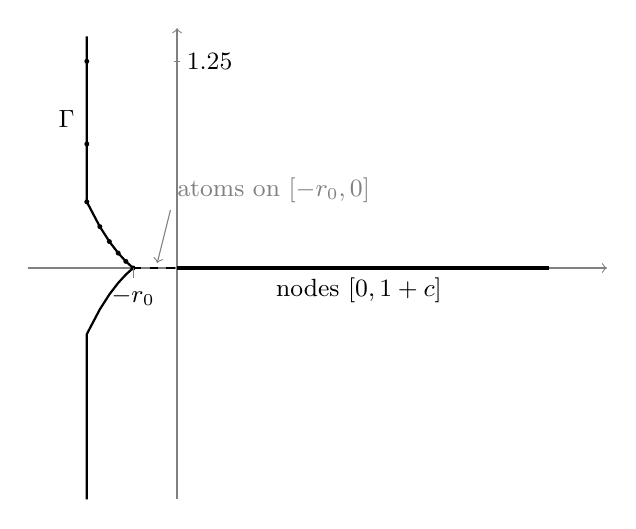
\begin{tikzpicture}[x=4.2cm,y=2.1cm]
  \draw[->,gray] (-0.45,0) -- (1.3,0);
  \draw[->,gray] (0,-1.4) -- (0,1.45);
  \draw[very thick] (0,0) -- (1.125,0);
  \node[below] at (0.55,0) {\small nodes $[0,1+c]$};
  \draw[thick,dashed] (-0.1329814,0) -- (0,0);
  \draw[thick] (-0.1329814,0) -- (-0.1548425,0.04) -- (-0.177904,0.09) -- (-0.2046703,0.16)
     -- (-0.2334108,0.25) -- (-0.2728752,0.4) -- (-0.2728752,0.75) -- (-0.2728752,1.25)
     -- (-0.2728752,1.4);
  \draw[thick] (-0.1329814,0) -- (-0.1548425,-0.04) -- (-0.177904,-0.09) -- (-0.2046703,-0.16)
     -- (-0.2334108,-0.25) -- (-0.2728752,-0.4) -- (-0.2728752,-0.75) -- (-0.2728752,-1.25)
     -- (-0.2728752,-1.4);
  \foreach \p in {(-0.1329814,0),(-0.1548425,0.04),(-0.177904,0.09),(-0.2046703,0.16),
     (-0.2334108,0.25),(-0.2728752,0.4),(-0.2728752,0.75),(-0.2728752,1.25)}
     {\fill \p circle (0.9pt);}
  \node[left] at (-0.28,0.9) {\small $\Gamma$};
  \draw[gray,->] (-0.02,0.35) node[above right=-1pt] {\small atoms on $[-r_0,0]$} -- (-0.06,0.03);
  \draw[gray] (-0.1329814,0) -- (-0.1329814,-0.06);
  \node[below] at (-0.1329814,-0.06) {\small $-r_0$};
  \node[right] at (0,1.25) {\small $1.25$};
  \draw[gray] (-0.01,1.25) -- (0.01,1.25);
\end{tikzpicture}
\caption{The scaled contour $\Gamma$ (vertices $v_0,\dots,v_7$ marked, vertical rays beyond
$v_7$ and $\bar v_7$), the interval $[-r_0,0]$ carrying the scaled poles of $F$, and the node
interval $[0,1+c]$. The horizontal scale is twice the vertical one.}
\label{fig:contour}
\end{figure}

\section{Proof of the theorem, the margin, and open points}\label{sec:proof}

This section combines the three estimates into the proof of \cref{thm:main}, explains why one
pair of certificates serves all four values of $k$, discusses how thin the margin is, and lists
what must still be verified before the theorem can be regarded as established.

\subsection{Proof of \texorpdfstring{\cref{thm:main}}{Theorem 1.1}}\label{subsec:main-proof}

Fix $k\in\{1,2,3,4\}$ and suppose that $\xi_k=X\in\Q$. For each $h\in16\N$,
\cref{prop:nonvanishing} (applied with this $X$) gives a set $I_h\subseteq\Com$ with
$\abs{I_h}\le1$ and $P^{\sep}_{I_h}(\xi_k)\ne0$. The number
$\den\bigl(P^{\sep}_{I_h}(\xi_k)\bigr)\cdot\abs{P^{\sep}_{I_h}(\xi_k)}$ is a positive integer, so
its logarithm is nonnegative. Both \cref{thm:arithmetic} and \cref{cor:decay-separated} are
uniform in the deletion, so they apply to $I_h$ and give
\begin{align*}
  0\le\log\den P^{\sep}_{I_h}(\xi_k)+\log\abs{P^{\sep}_{I_h}(\xi_k)}
   &\le\bigl(\cA-\cD_{\sep}+o(1)\bigr)h^2\\
   &\le\bigl(-0.000754+o(1)\bigr)h^2,
\end{align*}
since $\cA<3.5121304$ (\cref{thm:arithmetic}) and $\cD_{\sep}\ge3.5128848$
(\cref{cor:decay-separated}), and $3.5128848-3.5121304=0.0007544$. The right-hand side is negative
for large $h$, a contradiction. Hence $\xi_k\notin\Q$. \qed

\subsection{Uniformity in \texorpdfstring{$k$}{k} and the size of the margin}\label{subsec:margin}

The four values of $k$ are covered by the same two certificates. The arithmetic constant $\cA$
does not depend on $k$ (\cref{rem:A-k-independent}). In the analytic part, $k$ enters only
through the constant $C_1(k)$ of \cref{lem:contour} and through the positions of the atoms, which
form two progressions of step $1$ for every $k$; the node measure $\nu$, the contour, the trial
measure and the certified constants are the same for all $k$.

The proof uses the constants $\cD_{\alt}=3.5101772$ and $\cD_{\sep}=\cD_{\alt}+(\log2)/256$ of
\cref{thm:decay,cor:decay-separated}. With more digits of the certified bounds, the comparison
reads
\[
  \cD^{*}_{\alt}+\frac{\log2}{256}-\cA\ \ge\ 3.5101772515+0.0027076061-3.5121303756
  \ge0.00075448 ,
\]
where $\cD^{*}_{\alt}=3.5101772515\ldots$ is the certified rational lower bound of
\cref{prop:energy-certificate}; here the two lower bounds are truncated and the value of $\cA$ is
rounded up. The original archive, with its coarser energy certificate (lower bound
$3.5101522752$) and the rounded constants $3.5099$, $0.002707$ and $3.512131$, states the margin
$0.000476$; the certified value used here is $0.000754$.

With these certificates alone the comparison for the alternating geometry does not close:
$\cD^{*}_{\alt}-\cA=-0.0019531\ldots$\,. Since $\cD^{*}_{\alt}$ is a lower bound for the decay rate,
obtained from one contour and one trial measure, and $\cA$ is an upper bound for the denominator
rate, this negative difference does not prove that the alternating border fails for the numbers
$\xi_k$; it shows only that our two bounds do not suffice without the separation. For comparison,
\cite[\S12.1]{Litsey2026Lowner} reports an estimated deficit of about $0.0014$ for the alternating
border (\cref{subsec:context}); we have not reproduced that estimate.

The margin is about $0.02\%$ of the compared quantities. Every source of error in the
certificates is either exact rational arithmetic or enclosed rigorously
(Appendices~\ref{sec:arith-certificate} and~\ref{sec:error-analysis}), and the rigorous error
terms are many orders of magnitude below the margin; the danger is not rounding but a mistake in
the reduction of the asymptotic statements to the finite computations, or in their
implementation.

\emph{What the finite computations do and do not show.} No numerical experiment at accessible
sizes supports or contradicts the inequality $\cA<\cD_{\sep}$; the following facts, all taken from
the computations described in \cref{subsec:finite-checks} and in \emph{Reproducibility and formal
verification}, show how far the tested sizes are from the asymptotic regime.
\begin{enumerate}[(i)]
  \item \emph{Local bound.} For $h\le128$ the bound $2R_0+q$ of \cref{prop:nullspace} is attained
  at all but a few of the primes with $p^2>5N$ (at $118$ to $119$ of the $119$ primes for $h=128$).
  This says that the local bound is sharp at most primes of these sizes. It does not say that the
  constant $\cA$ is sharp: the theorem bounds the sum of the local bounds by the profile, and the
  primes below $\sqrt{5N}$ by $o(h^2)$.
  \item \emph{Distance to the limit on the arithmetic side.} For $h=128$ the primes with
  $p^2>5N$ contribute between $2.86$ and $2.92$ per $h^2$ to $\log\den$, depending on $k$, and
  the sums $\sum_p h\,e_\kappa(p/h)\log p$ of the profile over the same primes are larger by
  $0.011$ to $0.024$ per $h^2$, that is, by $15$ to $32$ times the margin. Both are far from
  $\cA=3.512\ldots$, because the primes $p\le\sqrt{5N}$, to which the proof allots $o(h^2)$, still
  contribute between $0.54$ and $0.59$ per $h^2$ at this size.
  \item \emph{The product itself.} Let $\operatorname{cont}P^{\sep}_\varnothing\in\Q$ be the
  content of the polynomial $P^{\sep}_\varnothing$. The quantity
  \[
    g(h,k)=h^{-2}\bigl(\log\den(\operatorname{cont}P^{\sep}_\varnothing)
    +\log\abs{P^{\sep}_\varnothing(\xi_k)}\bigr),
  \]
  computed for $h\le96$ and all $k$, lies between $-0.176$ and $+0.010$; it is positive for $k=3$
  at $h=80$ ($+0.0030$) and $h=96$ ($+0.0091$). \TRENDEXTRA{} These values are $0.01$ to $0.2$ per $h^2$ away from the
  limiting bound $\cA-\cD_{\sep}\le-0.000754$, they are not monotone in $h$, and they neither
  confirm nor contradict it. (The content of the polynomial bounds the denominator at every
  rational point with denominator prime to the primes concerned; it is not the denominator at one
  point.)
  \item \emph{The separation is invisible at these sizes.} For rational $X$, the numerators of
  $P^{\sep}_I(X)$ and $P^{\alt}_I(X)=2^{m(m-1)}P^{\sep}_I(X)$ coincide as long as
  $m(m-1)\le-v_2(P^{\sep}_I(X))$. The latter is $O(h\log h)$ but large: for $k=1$ and $h=64$ the
  $2$-adic Gauss valuation of the polynomial $P^{\sep}_\varnothing$ is $-752$, against
  $m(m-1)=12$. The entrywise bound $-v_2\le2n\lfloor\log_2(5N)\rfloor$ (for $X$ with odd
  denominator) is smaller than $m(m-1)$ only for $h\ge8192$; this is an upper estimate for the
  size at which the separation must change $\den\cdot\abs P$, and the true threshold, which we
  do not know, is lower.
\end{enumerate}
The contradiction is therefore asymptotic in a strong sense, and the evidence for it is the
written reduction of the two asymptotic statements (\cref{thm:arithmetic,thm:decay}) to the two
finite certificates, not any experiment. On the analytic side, $V$ is nearly constant on the part
of the contour that carries $\mu$ (\cref{subsec:trial-measure}); this suggests, heuristically and
without proof, that the certified decay is close to the best value obtainable from this contour
by the criterion of \cref{prop:energy-criterion}.

\begin{remark}[Pairwise irrationality]\label{rem:pairwise}
Independently of the rest of the paper, \eqref{eq:pair-sum} shows that $\xi_1+\xi_4$ and
$\xi_2+\xi_3$ are nonzero algebraic multiples of $\pi^2$, hence transcendental by Lindemann's
theorem. So at least one number in each pair is irrational. This weaker statement is all that
that we found in the literature (\cref{subsec:context}). The Lean package proves formally the still weaker
statement that at least one of $\xi_1,\dots,\xi_4$ is irrational, from
$\xi_1+\xi_2+\xi_3+\xi_4=2\pi^2$.
\end{remark}

\begin{remark}[Irrationality measures]\label{rem:no-measure}
An irrationality measure would require the decay bound on a neighbourhood of $\xi_k$ of size
$\exp(-\rho h^2)$, uniformly in $X$, as in~\cite[\S\S6, 11]{Litsey2026Lowner}. With a margin of
$0.00075$ per $h^2$ any resulting exponent would be enormous, and we have not pursued this.
\end{remark}

\subsection{Open points}\label{subsec:open-points}

\Cref{tab:status} records the status of each step. We list the points that, in our judgement,
must be settled before \cref{thm:main} can be regarded as established. None of them is known to
fail.
\begin{enumerate}[(O1)]
  \item \emph{Human review.} No human mathematician has checked the argument or the certificates.
  All reviews and recomputations so far were performed by an AI
  system and are not independent certification.
  \item \emph{Steps without any review.} \Cref{prop:nonvanishing} and the prime-number-theorem
  bookkeeping in the proof of \cref{thm:arithmetic} have been checked only in the course of
  writing this paper; the nonvanishing statement is supported at small sizes by the absence of
  rational roots (\cref{rem:nonvanishing}).
  \item \emph{Candidate steps reviewed only internally.} The polar congruences
  (\cref{lem:two-layer}), the simultaneous nullspace bound (\cref{prop:nullspace}), the contour
  representation (\cref{lem:contour}) and the energy criterion (\cref{prop:energy-criterion})
  were checked in the AI-internal audit, partly against exact valuations at finite $h$;
  the proofs written here should be read by a referee, in particular the uniformity of Step~4 of
  \cref{prop:energy-criterion} near the atoms closest to the origin and on the vertical rays.
  \item \emph{The constant $p_0$ and the excluded primes.} \Cref{def:block-types} excludes the
  finitely many primes $p\le p_0$, where $p_0>120$ depends on the chosen bases; only its
  finiteness is used, and it has not been computed. The exclusion is not a formality: primes at
  which a fibre block has smaller rank modulo $p$ than over $\Q$ do occur in the finite tests
  (four cases, the largest $p=31$ at $h=128$, \cref{subsec:finite-checks}); all of them are below
  $120$ and none contradicts \cref{prop:nullspace}, but the set of such primes over all the types
  that occur has not been determined.
  \item \emph{Profile lemmas.} \Cref{lem:profile-bound,lem:profile-structure}, on which the exact
  integration of $\cA$ rests, are proved here and have had no review; a breakpoint missing
  from~\eqref{eq:breakpoints} would change the computed value of $\cA$ without any program
  noticing, except through the affinity checks of \cref{subsec:arith-checks}.
  \item \emph{Implementations.} Each certificate has two implementations (\cref{sec:arith-certificate,sec:error-analysis}),
  all written by AI systems; none has been read line by line by a second party.
  \item \emph{Formal verification.} The Lean development proves only the final deduction,
  conditionally on the estimates (see \emph{Reproducibility and formal verification}).
\end{enumerate}


\appendix
\section{The arithmetic certificate}\label{sec:arith-certificate}

This appendix documents the computation behind \cref{prop:A-value}, the exact value of the
arithmetic constant $\cA$ used in \cref{thm:arithmetic}, and the checks it has passed. It
describes how the type data are computed, how the profile is integrated exactly, and how the local
bound of \cref{prop:nullspace} was tested against exact valuations at finite $h$.

\subsection{Type data}\label{subsec:type-data}

For each $\kappa\in\{\frac15,\dots,\frac45\}$ and each type
$(\kappa,\mathcal L^\Row,\mathcal L^\Col,\varepsilon)$ of the alternating form of
\cref{def:profile} (common digits $\{0,\dots,\gamma-1\}$, border digits $\{\gamma,\dots,T-1\}$ alternating
between rows and columns, $T\le23$), the program computes the rational numbers $V_l,W_l$ of
\eqref{eq:VW-def}, the block $A_\tau$, its rank over $\Q$, bases of its left and right null spaces
by exact row reduction, the images of these null spaces under the moment map, and the lines they
span. Over the whole range $1/20\le u\le45/8$ about a thousand types occur ($1042$
according to the AI-internal audit), and no null space has a two-dimensional moment image, so the
convention of \cref{def:block-types}(ii) for two-dimensional images is never used.

\begin{example}\label{ex:profile-x4}
Let $\kappa=\frac15$ and $u=4$. For $t\in[0,1)$ a fibre has one common digit; for
$t\in[1,\frac98)$ one border digit; for larger $t$ none. Here $\varepsilon(t)=(\mathbf1[t>\frac45],0)$.
A common singleton has $A=[W_0]$ with $W_0=-\varepsilon_1/\kappa^2$: rank $0$ for $t<\frac45$, with
left and right null vector $(1)$ of moment $(1,V_0)=(1,0)$, and rank $1$ for $\frac45<t<1$. A border
singleton is a $1\times0$ or $0\times1$ block of rank $0$ whose null vector has moment
$(1,1/\kappa)=(1,5)$; half of these fibres are rows and half columns. Hence $\rho=0.2$,
$\alpha=\beta=0.8+0.0625$, the line $\Q(1,0)$ has $\alpha_\Lambda=\beta_\Lambda=0.8$ and the line
$\Q(1,5)$ has $\alpha_\Lambda=\beta_\Lambda=0.0625$. Thus $q=\min(0.8625,\,0.8625,\,0.125,\,1.6)=0.125$
and $e_{1/5}(4)=0.4+0.125=0.525$. Without the line bound one would get $0.4+0.8625$.
\end{example}

\Cref{tab:profile} shows the profile at a few points. It falls from about $2.1$, close to
the trivial value $2+c$, to $0$, but not monotonically (for $\kappa=\frac25$ it is $2.000$ near
$u=0.5$ and $2.050$ near $u=0.75$); for $\kappa\ge\frac25$ it vanishes for $u\ge3$, while for
$\kappa=\frac15$ it stays positive up to $u=45/8$, which explains the larger integral in that
class.

\begin{table}[ht]
\centering
\small
\setlength{\tabcolsep}{4.6pt}
\begin{tabular}{@{}lcccccccccccc@{}}
\toprule
$u$ & $0.05$ & $0.1$ & $0.25$ & $0.5$ & $0.75$ & $1$ & $1.5$ & $2$ & $3$ & $4$ & $5$ & $5.5$\\
\midrule
$\kappa=\frac15$ & 2.110 & 2.075 & 2.050 & 2.025 & 2.000 & 1.850 & 1.525 & 1.325 & 0.925 & 0.525 & 0.125 & 0.025\\
$\kappa=\frac25$ & 2.105 & 2.075 & 2.025 & 2.000 & 2.050 & 1.450 & 0.925 & 0.525 & 0 & 0 & 0 & 0\\
$\kappa=\frac35$ & 2.100 & 2.085 & 2.000 & 2.000 & 2.000 & 1.250 & 0.625 & 0.125 & 0 & 0 & 0 & 0\\
$\kappa=\frac45$ & 2.100 & 2.0875 & 2.000 & 2.000 & 2.000 & 1.250 & 0.625 & 0.125 & 0 & 0 & 0 & 0\\
\bottomrule
\end{tabular}
\caption{The profile $e_\kappa$ at the points $u+10^{-6}$ for the displayed $u$, rounded to three
decimals (the entry $2.0875$ is given with four). The trivial
entrywise bound corresponds to the constant $2+c=2.125$.}
\label{tab:profile}
\end{table}

\subsection{Exact integration}\label{subsec:exact-integration}

For each $\kappa$ the interval $[1/20,45/8]$ is cut at the points~\eqref{eq:breakpoints} lying
inside it, giving $122$, $123$, $122$ and $122$ cells for $\kappa=\frac15,\dots,\frac45$. On a cell
$(l,r)$ the original program evaluates all candidate functions
$2\rho+\alpha$, $2\rho+\beta$ and $2\rho+\alpha+\beta-\alpha_\Lambda-\beta_\Lambda$ at the interior
points $(2l+r)/3$ and $(l+2r)/3$, reconstructs each as an affine function, adds the pairwise
intersection points inside the cell as further cuts, and integrates the minimum exactly by
evaluating it at the midpoint of each sub-cell. Adding $\frac{2+c}{20}=\frac{17}{160}$ for the
range below $u=1/20$ and averaging over $\kappa$ gives
\[
  \cA=\frac{304227995343501721142691896310988016794079029050925423}
           {86622067750624596685118168422516024981216422248448000}.
\]
The inequality $\cA<3512131/10^6$ is checked in rational arithmetic. No quadrature or floating
point enters.

\subsection{Checks of the arithmetic computation}\label{subsec:arith-checks}

\begin{enumerate}[(a)]
  \item \emph{Separated geometry.} The original program integrates the analogous profile for the
  separated geometry (border rows on $[1,1+c/2)$, columns on $[1+c/2,1+c)$, no parity averaging)
  and obtains exactly the same rational number. This is consistent with \cref{cor:separation},
  which makes the odd-prime denominators of the two geometries equal.
  \item \emph{Recomputation from the description.} In the AI-internal audit the profile was
  reimplemented from the mathematical description, with the piece lengths carried symbolically
  as affine functions of $u$, the breakpoints generated independently as the intersections of
  the lines $0,u,\kappa u,u/2,1-ju,1+c-ju$, and the constancy of the combinatorial type and of the
  affine candidates asserted at two points of every interval. It reproduces the four integrals
  and $\cA$ exactly. Using the best labelling of two-dimensional moment images instead of the
  coordinate lines gives the same value, since such images do not occur.
  \item \emph{Affinity.} We evaluated, for each of the $489$ cells of the original program, the
  candidate functions at the three further points $l+\frac1{11}(r-l)$, $\frac{l+r}2$,
  $l+\frac9{10}(r-l)$ and compared them with the affine reconstruction: all agree exactly.
  Together with the two points of the reconstruction this makes five points per cell. Such a test
  supports \cref{lem:profile-structure} but cannot replace it: finitely many points do not
  exclude a breakpoint inside a cell.
  \item \emph{Polar congruences.} The congruences of \cref{lem:two-layer} were checked on
  $312{,}120$ matrix entries (\cref{subsec:polar}).
\end{enumerate}

\subsection{Finite tests of the local bound}\label{subsec:finite-checks}

\Cref{prop:nullspace} can be tested at finite $h$ by computing the exact polynomial
$P^{\alt}_I(X)$, or its value at a rational point, and comparing the exponent $e_p$ with the
prediction $2R_0+q$ computed from the actual fibres. Since $p_0$ has not been computed, we cannot
say which of the primes tested are ordinary; those below $120$, where the exponents are largest,
are not. The tests therefore check the formula of the proposition, and the mechanism of its proof,
partly at primes that the proof excludes. Recall from
\cref{rem:bad-primes} that a prime is \emph{bad} if some fibre block has smaller rank modulo $p$
than over $\Q$.
\begin{enumerate}[(a)]
  \item \emph{Rational data, value at a point.} We compared $e_p(P^{\alt}_\varnothing(1/7))$ with
  $2R_0+q$, computed over $\Q$ exactly as in \cref{prop:nullspace}, at every prime
  $p\notin\{5,7\}$ with $\sqrt{5N}<p\le5N$, for $h\in\{16,32,48,64,80,96,128\}$ and all $k$
  ($1836$ comparisons): no violation, at bad primes or elsewhere; equality at $1810$ primes, and
  at $117$ to $119$ of the $119$ primes when $h=128$. (The sizes $h\in\{32,48,64,96\}$ are run by
  a program of the package; the others were added for this revision.)
  \item \emph{Data modulo $p$, Gauss valuations.} The AI-internal audit compared the Gauss
  valuations of the exact polynomials $P^{\alt}_I(X)$ (\cref{rem:gauss}) with the number
  $2R'_0+\rank_{\Fp}K$ in which every rank is computed modulo $p$: $R'_0$ is the sum of the ranks
  over $\Fp$ of the fibre blocks, and $K$ is the pairing between their null spaces over $\Fp$.
  At a prime that is not bad, $R'_0=R_0$ and this is the intermediate bound in the proof of
  \cref{prop:nullspace}. The comparison was made at every odd prime $p\ne5$ with $p^2>5N$, for
  $h\in\{16,32,48,64,80,96,128\}$ and all $k$, and with the deletions $\{0\}$ and $\{h-1\}$ for
  $h\in\{32,48\}$: no violation at any prime that is not bad.
  \item \emph{Bad primes.} Four bad primes occur in the tests of (b) without deletion
  (\cref{tab:bad-primes}); the prime $17$ at $h=32$, $k=1$ is also bad for the two deletions. At
  two of the four, $e_p$ exceeds the number computed modulo $p$: by $3$ at $h=16$, $k=3$, $p=11$,
  and by $4$ at $h=128$, $k=3$, $p=31$, the largest size tested. As explained in
  \cref{rem:bad-primes}, this contradicts no statement of this paper: the number computed modulo
  $p$ is not the bound of \cref{prop:nullspace}, which is stated with ranks over $\Q$ and for
  $p>p_0$ only. With the rational data the inequality $e_p\le2R_0+q$ holds at all four bad primes,
  for the Gauss valuation and at the points $X\in\{0,1,\frac17,\frac23,\frac3{11}\}$. The rank
  drops are explicit: for $p=31$ the block of the type with four common digits, $\kappa=\frac35$ and
  $\varepsilon=(1,1)$ is a $4\times4$ matrix of rank $4$ whose determinant has numerator divisible
  by $31$, and this type occurs in the eleven fibres $20\le\iota\le30$; for $p=11$ and $p=13$ it
  is the $1\times1$ block $W_0=4-\kappa^{-2}$, equal to $\frac{11}9$ and $\frac{39}{16}$; for
  $p=17$ a $2\times2$ block of determinant $\frac{17}3$.
  \item \emph{Comparison with the profile.} In the tests of (a) the prediction $2R_0+q$ exceeds
  $h\,e_\kappa(p/h)$ by at most $0.8$, and the exponent $e_p$ itself exceeds $h\,e_\kappa(p/h)$ at
  $56$ of the $1836$ primes (for instance $98>97.2$ at $h=48$, $k=1$, $p=41$). So the profile does
  not dominate prime by prime; this is consistent with \cref{lem:profile-bound}, whose constant
  $C_0$ cannot be taken to be $0$. What holds in all $28$ cases is the inequality between the
  sums: $\sum_p(2R_0+q)\log p<\sum_ph\,e_\kappa(p/h)\log p$ over the primes tested, the difference
  being between $0.0099$ and $0.1754$ per $h^2$ and decreasing with $h$ for each $k$.
\end{enumerate}

\begin{table}[ht]
\centering
\small
\begin{tabular}{@{}ccccccc@{}}
\toprule
$h$ & $k$ & $p$ & $e_p$ & computed modulo $p$ & $2R_0+q$ over $\Q$ & $h\,e_\kappa(p/h)$\\
\midrule
$16$ & $2$ & $13$ & $28$ & $28$ & $28$ & $29.0$\\
$16$ & $3$ & $11$ & $29$ & $26$ & $33$ & $32.9$\\
$32$ & $1$ & $17$ & $64$ & $64$ & $66$ & $66.0$\\
$128$ & $3$ & $31$ & $253$ & $249$ & $260$ & $260.5$\\
\bottomrule
\end{tabular}
\caption{The four bad primes met in the finite tests (no deletion). Here $e_p$ is the exponent of
$p$ in the denominator of the content of $P^{\alt}_\varnothing$, and the fifth column is the
number $2R'_0+\rank_{\Fp}K$ of test~(b).}
\label{tab:bad-primes}
\end{table}

These tests concern the inequality of \cref{prop:nullspace}, not the asymptotic constant: at
these sizes the contribution of the small primes is still of the same order as that of the
others (\cref{subsec:margin}).

\section{The contour and the trial measure}\label{sec:contour-and-measure}

This appendix specifies the polygon $\Gamma$ and the trial measure $\mu$ to which the energy
criterion (\cref{prop:energy-criterion}) is applied in \cref{prop:energy-certificate}, and records
the properties of $\mu$ that the criterion requires. The data are stored in the file \file{trial.json} of the original archive (SHA-256
\texttt{a4da00b3a51e1d41\ldots c499c}); all coordinates are rational with common denominator
$7\,054\,320\,000\,000$ and all masses are integers divided by $10^{12}$.

\subsection{The polygon}\label{subsec:polygon}

The upper half $\Gamma^+$ of $\Gamma$ is the polygonal path through the vertices of
\cref{tab:vertices}, followed by the vertical ray $v_7+i[0,\infty)$; $\Gamma=\Gamma^+\cup\overline{\Gamma^+}$.
The verifier checks that all vertices have negative real part, that $v_0$ is real and that the
ordinates increase strictly, so $\Gamma$ is a simple curve in $\{\operatorname{Re}z<0\}$ meeting
$\R$ only at $v_0=-r_0$.

\begin{table}[ht]
\centering
\small
\begin{tabular}{@{}cll@{}}
\toprule
vertex & real part & imaginary part\\
\midrule
$v_0$ & $-664907/5000000=-0.1329814$ & $0$\\
$v_1$ & $-61937/400000=-0.1548425$ & $1/25$\\
$v_2$ & $-11119/62500=-0.177904$ & $9/100$\\
$v_3$ & $-2046703/10000000=-0.2046703$ & $4/25$\\
$v_4$ & $-583527/2500000=-0.2334108$ & $1/4$\\
$v_5$ & $-170547/625000=-0.2728752$ & $2/5$\\
$v_6$ & $-170547/625000$ & $3/4$\\
$v_7$ & $-170547/625000$ & $5/4$\\
\bottomrule
\end{tabular}
\caption{Vertices of the upper half of the scaled contour $\Gamma$.}
\label{tab:vertices}
\end{table}

\subsection{The trial measure}\label{subsec:trial-measure}

The trial measure $\mu$ is a sum of $238$ uniform measures on segments:
\begin{itemize}
  \item $34$ consecutive segments of equal length partitioning $[-r_0,0]$, carrying total mass
  $0.2659627999\ldots$, with density between $2-6\cdot10^{-10}$ and $2-3\cdot10^{-11}$;
  \item $102$ segments of length between $0.0038$ and $0.0040$ on the edges of $\Gamma^+$ up to
  height $0.377$, with densities between $0.028$ and $1.92$ and total mass
  $0.3982686000\ldots$;
  \item the $102$ complex conjugate segments, with the same masses.
\end{itemize}
The verifier checks exactly: every mass is positive, the total mass is $17/16=\lambda$, the
measure is invariant under conjugation, every segment lies on an edge of $\Gamma$ or on
$[v_0,0]$, and every endpoint $w$ satisfies $\abs{\operatorname{Re}w}+\abs{\operatorname{Im}w}\le1$,
so $\operatorname{supp}\mu\subset\{\abs w\le1\}$. Thus $\mu$ satisfies the hypotheses of
\cref{prop:energy-criterion}.

The trial measure was produced by a floating-point optimizer (a discretized quadratic program for
the constrained equilibrium of \cref{rem:energy-meaning}) and then rounded to rationals; the
certificate does not depend on how it was found. In the AI-internal audit, half of the $3639$
cell endpoints of the certificate have a value of $V$ within about $1.5\cdot10^{-4}$ of the
minimum. These endpoints are concentrated on the part of $\Gamma$ that carries $\mu$, of height at
most $0.377$; above it $V$ increases, up to about $4.12$ on the finite part of the contour. So $V$
is nearly constant on the support of $\mu$ in $\Gamma$, as it would be for an equilibrium measure;
this suggests that $\mu$ is close to optimal for this contour, but we have not proved it and do
not use it. The audit also finds $V<\theta$ on all but about $6\cdot10^{-5}$ of the interval
$[-r_0,0]$, so the term $4J\approx-0.239$ matters.

\section{Exact formulas for potentials and energies}\label{sec:exact-formulas}

This appendix collects the closed forms used by the energy certificate
(\cref{sec:error-analysis}): the potential of a uniform segment and its second derivative along a
line, the mutual energy of two segments, and the energy of the node measure $\nu$. Throughout, $\operatorname{Log}$ is the principal branch, and for a segment $[a,b]\subset\C$ we
write $\mathrm u_{[a,b]}$ for the uniform probability measure on it.

\subsection{Potential of a segment}\label{subsec:segment-potential}

\begin{lemma}\label{lem:segment-potential}
Let $a\ne b$, $v=b-a$ and $u=(z-a)/v$. Then
\[
  \pot{\mathrm u_{[a,b]}}(z)=1-\log\abs v-\operatorname{Re}\bigl[u\operatorname{Log}u-(u-1)\operatorname{Log}(u-1)\bigr],
\]
with $0\operatorname{Log}0=0$. In particular the potential of a segment-regular measure is continuous,
with modulus of continuity $O(\delta\log(1/\delta))$ on compact sets.
\end{lemma}

\begin{proof}
$\pot{\mathrm u_{[a,b]}}(z)=-\log\abs v-\int_0^1\log\abs{u-\tau}\,\dd\tau$. If
$\operatorname{Im}u\ne0$, then $u-\tau$ stays in one open half-plane, $\operatorname{Log}(u-\tau)$ is
continuous in $\tau$, and
$\int_0^1\operatorname{Log}(u-\tau)\,\dd\tau=u\operatorname{Log}u-(u-1)\operatorname{Log}(u-1)-1$; take real
parts. For real $u$ the formula follows by continuity, since
$\operatorname{Re}(u\operatorname{Log}u)=u\log\abs u$ for $u\in\R$. The modulus of continuity
follows from that of $t\log\abs t$.
\end{proof}

\begin{lemma}[Uniform continuity on the plane]\label{lem:uniform-continuity}
Let $\mu_1$ be a segment-regular measure. There is a constant $C(\mu_1)$ such that
$\abs{\pot{\mu_1}(z)-\pot{\mu_1}(z')}\le C(\mu_1)\,\delta\log(1/\delta)$ for all $z,z'\in\C$ with
$\abs{z-z'}\le\delta\le\frac12$.
\end{lemma}

\begin{proof}
Let $K$ be the compact set of points at distance at most $2$ from $\operatorname{supp}\mu_1$. If
$z,z'\in K$, the estimate is the one of \cref{lem:segment-potential} on $K$. Otherwise one of the
two points is at distance more than $2$ from the support, and then the whole segment $[z,z']$, of
length at most $\frac12$, is at distance at least $1$ from it. On the set of points at distance
at least $1$ from the support, $\pot{\mu_1}$ is smooth with
$\abs{\nabla\pot{\mu_1}(z)}\le\int\abs{z-w}^{-1}\,\dd\abs{\mu_1}(w)\le\abs{\mu_1}(\C)$, so
$\abs{\pot{\mu_1}(z)-\pot{\mu_1}(z')}\le\abs{\mu_1}(\C)\,\delta\le\abs{\mu_1}(\C)\,\delta\log(1/\delta)/\log2$.
\end{proof}

Along a straight cell $z(t)=z_0+t(z_1-z_0)$ not meeting the endpoints of the segments, the second
derivative of the potential of a signed combination $\eta=\sum_j\mathfrak m_j\mathrm u_{[a_j,b_j]}$ is
\begin{equation}\label{eq:second-derivative}
  \frac{\dd^2}{\dd t^2}\pot\eta(z(t))=-\operatorname{Re}\Bigl[(z_1-z_0)^2\sum_{e}\frac{\gamma_e}{z(t)-e}\Bigr],
  \qquad\gamma_e=\sum_{j:\,a_j=e}\frac{\mathfrak m_j}{b_j-a_j}-\sum_{j:\,b_j=e}\frac{\mathfrak m_j}{b_j-a_j},
\end{equation}
the sum running over all segment endpoints $e$. Indeed the complex potential
$\Theta(z)=\int\operatorname{Log}(z-w)\,\dd\eta(w)$ satisfies
$\Theta''(z)=\sum_j\mathfrak m_j\bigl(\frac1{z-a_j}-\frac1{z-b_j}\bigr)/(b_j-a_j)$, and
$\pot\eta=-\operatorname{Re}\Theta$. The field $(1-\varepsilon_0)\pi\abs{\operatorname{Im}z}$ is affine
along cells contained in a closed half-plane, so~\eqref{eq:second-derivative} is also the second
derivative of $V$ along the cells of $\Gamma^+$ and of $[-r_0,0]$, with $\eta=\mu-\nu$.

\subsection{Energies}\label{subsec:energy-formulas}

Let $\mathcal G(z)=\frac12z^2\operatorname{Log}z-\frac34z^2$, so that $\mathcal G''=\operatorname{Log}$.

\begin{lemma}\label{lem:segment-energies}
(a) $I(\mathrm u_{[a,b]})=\frac32-\log\abs{b-a}$.

(b) Let $[a,b]$ and $[c',d]$ be segments with $v=b-a$ and $w=d-c'$, and suppose that the four
differences $b-c'$, $a-d$, $a-c'$, $b-d$, after multiplication by a common $\epsilon\in\{\pm1,\pm i\}$,
lie in the closed right half-plane. Then
\[
  I\bigl(\mathrm u_{[a,b]},\mathrm u_{[c',d]}\bigr)
  =-\operatorname{Re}\frac{\mathcal G(\epsilon(b-c'))+\mathcal G(\epsilon(a-d))-\mathcal G(\epsilon(a-c'))-\mathcal G(\epsilon(b-d))}{\epsilon^2vw}.
\]
\end{lemma}

\begin{proof}
(a) is the case $a=0$, $b=\ell$ of $\int_0^1\int_0^1-\log(\ell\abs{\tau-\tau'})\,\dd\tau\dd\tau'=\frac32-\log\ell$.
(b) The differences $\epsilon(a+\tau v-c'-\tau'w)$, $\tau,\tau'\in[0,1]$, fill the parallelogram
spanned by the four rotated corner differences, which lies in the closed right half-plane, where
$\operatorname{Log}$ is continuous away from $0$. Since
$\partial_\tau\partial_{\tau'}\mathcal G(\epsilon(a+\tau v-c'-\tau'w))=-\epsilon^2vw\operatorname{Log}(\epsilon(\cdots))$,
integrating over the unit square gives
$\iint\operatorname{Log}(\epsilon(\cdots))=[\cdots]/(\epsilon^2vw)$, and
$\operatorname{Re}\operatorname{Log}(\epsilon y)=\log\abs y$. If the parallelogram contains $0$ the
formula follows by continuity.
\end{proof}

\begin{lemma}\label{lem:Inu}
For $a>0$, $I\bigl(\mathrm{Leb}|_{[0,a]}-\mathrm{Leb}|_{[a,2a]}\bigr)=4a^2\log2$. For the node
measure~\eqref{eq:nu-def} with $c=\frac18$,
\begin{align*}
  I(\nu)&=\frac32+\frac{3c}2+\frac{3c^2}8+\frac{c^2}4\log c-\frac{(1+c)^2}2\log(1+c)\\
  &=\frac{867}{512}+\frac{483}{256}\log2-\frac{81}{64}\log3=1.6107019792\ldots .
\end{align*}
\end{lemma}

\begin{proof}
By \cref{lem:segment-energies}(a) an interval of length $\ell$ with density $1$ has energy
$\ell^2(\frac32-\log\ell)$, and for real intervals
$\int_\alpha^\beta\int_\gamma^\delta-\log(y-x)\,\dd y\,\dd x=-\bigl[\mathcal G(\delta-\alpha)-\mathcal G(\delta-\beta)
-\mathcal G(\gamma-\alpha)+\mathcal G(\gamma-\beta)\bigr]$ when $\beta\le\gamma$, with $\mathcal G(0)=0$. For the first claim,
the mutual energy of $[0,a]$ and $[a,2a]$ is $-(\mathcal G(2a)-2\mathcal G(a))=a^2(\frac32-\log a-2\log2)$, and
$2a^2(\frac32-\log a)-2a^2(\frac32-\log a-2\log2)=4a^2\log2$. For the second,
$I(\nu)=\frac32+\frac{c^2}4(\frac32-\log c)-\bigl(\mathcal G(1+c)-\mathcal G(1)-\mathcal G(c)\bigr)$, which simplifies as
displayed.
\end{proof}

\section{The energy certificate}\label{sec:error-analysis}

This appendix explains why the numbers in \cref{prop:energy-certificate} are rigorous bounds.
There are two implementations: the ball-arithmetic computation made during the AI-internal
audit, which gives the certified values used in the proof, and the original fixed-point verifier, which
uses a coarser cover and gives slightly weaker bounds. Both rest on the formulas of
\cref{sec:exact-formulas} and on the following interpolation lemma.

\begin{lemma}\label{lem:chord}
Let $f$ be continuous on $[0,1]$ and $C^2$ on $(0,1)$ with
$\abs{f''(t)}\le K_0+K_1/t+K_2/(1-t)$ for constants $K_0,K_1,K_2\ge0$. Then
$\abs{f(t)-((1-t)f(0)+tf(1))}\le K_0/8+(K_1+K_2)/\e$ for $t\in[0,1]$.
\end{lemma}

\begin{proof}
Let $g$ be $f$ minus its chord and
$\phi(t)=\frac{K_0}2t(1-t)-K_1t\log t-K_2(1-t)\log(1-t)\ge0$. Then $\phi''=-K_0-K_1/t-K_2/(1-t)$,
so $\phi\pm g$ is concave on $(0,1)$, continuous on $[0,1]$ and zero at the endpoints, hence
nonnegative. Finally $\max\phi\le K_0/8+(K_1+K_2)\max(-t\log t)=K_0/8+(K_1+K_2)/\e$.
\end{proof}

On a straight cell from $z_0$ to $z_1$ that contains no segment endpoint in its interior,
\eqref{eq:second-derivative} gives
$\abs{\frac{\dd^2}{\dd t^2}V}\le\abs{z_1-z_0}^2\sum_e\abs{\gamma_e}/\abs{z(t)-e}$. An endpoint $e$ of
the cell contributes $K_1/t$ or $K_2/(1-t)$ with $K_{1,2}=\abs{\gamma_e}\abs{z_1-z_0}$; any other
segment endpoint contributes to $K_0$ through a lower bound for its distance to the cell.

\subsection{The certified computation}\label{subsec:energy-recomputation}

The AI-internal audit rebuilt the certificate from the definitions, with Arb ball arithmetic at
$256$ bits and exact rational geometry; every asserted inequality is checked on ball endpoints or
in exact rational arithmetic, and the program stops if one fails.
\begin{itemize}
  \item \emph{Data.} The hypotheses on $\Gamma$ and $\mu$ listed in \cref{sec:contour-and-measure}
  are checked exactly; moreover $\operatorname{supp}\mu\subset\{\abs w\le R_\mu\}$ with
  $R_\mu\le0.4618$.
  \item \emph{Contour.} The values of $V$ are enclosed with \cref{lem:segment-potential}. Each
  edge of $\Gamma^+$ is split at the segment endpoints lying on it and bisected until the bound of
  \cref{lem:chord} is at most $10^{-6}$ ($3639$ cells). The minimum over cells of
  $\min(V(z_0),V(z_1))$ minus this bound, minus a strictness buffer $10^{-9}$, gives
  $\theta=2.1001432662\ldots$; the smallest endpoint value of $V$ is $2.1001436\ldots$, the median
  over the cell endpoints is $2.1002856\ldots$ and the largest is $4.1198\ldots$\,. The endpoints
  are concentrated on the part of $\Gamma$ carrying $\mu$ (height at most $0.377$), where $V$ is
  therefore nearly constant; it is not nearly constant on the whole contour.
  \item \emph{Vertical rays.} For $\operatorname{Re}z<0$ and $w\ge0$ one has $\abs{z-w}\ge\abs z$,
  so $\pot\nu(z)\le-\lambda\log\abs z$; and $\pot\mu(z)\ge-\lambda\log(\abs z+R_\mu)$. Hence, on the
  upward ray from $v_7$, with $\upsilon=\operatorname{Im}z$,
  \[
    V(z)\ge(1-\varepsilon_0)\pi\upsilon-\lambda\log\Bigl(1+\frac{R_\mu}{\abs z}\Bigr)
    \ge(1-\varepsilon_0)\pi\upsilon-\frac{\lambda R_\mu}\upsilon ,
  \]
  which increases with $\upsilon$ and is at least $3.5344>\theta$ at $\upsilon=\frac54$. The lower ray follows
  by symmetry.
  \item \emph{Atom term.} The interval $[v_0,0]$ is covered by $760$ cells with the same
  tolerance. On each cell the linear function taking the values
  $V(z_j)-\theta-\text{bound}$ at the endpoints lies below $V-\theta$ by \cref{lem:chord}; the
  integral of its negative part is computed exactly (a trapezoid if both endpoint values are
  negative, a triangle if one is), giving $J\ge-0.0598567117\ldots$. The lower chord is below
  $0$ on all but about $6\cdot10^{-5}$ of the interval.
  \item \emph{Energies.} $I(\mu)$ is the sum over pairs of segments of the products of the masses
  and of the pair energies of \cref{lem:segment-energies}, with the branch condition checked
  exactly for each pair; the resulting ball is $2.32390232137306459\ldots$ with radius below
  $10^{-71}$. $I(\nu)$ is enclosed from \cref{lem:Inu}, and agrees with the pair-energy formula.
  \item \emph{Conclusion.} The rational lower bound for $2\lambda\theta+4J-I(\mu)+I(\nu)$ is
  $\cD^{*}_{\alt}=3.5101772515\ldots$; adding $(\log2)/256$ gives $3.5128848577\ldots$, which exceeds
  $\cA$ by $0.0007544821\ldots$. The constants $\cD_{\alt}=3.5101772$ and
  $\cD_{\sep}\ge3.5128848$ used in the proof are truncations of these numbers.
\end{itemize}

\subsection{The original fixed-point verifier}\label{subsec:fixed-point}

The original verifier represents approximate values as integers in units of $\mathsf S^{-1}$,
$\mathsf S=2^{100}$, and computes $\log$ of positive rationals, $\arg$ of nonzero Gaussian
rationals and $\pi$ with error at most $\mathsf E/\mathsf S$, $\mathsf E=10^6$
($\approx7.9\cdot10^{-25}$).
\begin{itemize}
  \item $\log(x/y)$: write $x/y=2^jv$ with $1\le v<2$ and $\abs j<1000$ (asserted), and use
  $\log v=2\sum_{i\ge0}u^{2i+1}/(2i+1)$, $u=(v-1)/(v+1)\le\frac13$, truncated after $64$ terms with
  every product floored. The rounding errors add up to at most $384$ units and the tail is below
  one unit since $3^{-129}<2^{-100}$; with $\log2$ computed in the same way, the error is at most
  $385(1+\abs j)<\mathsf E$ units.
  \item $\arctan u$ for $0\le u\le\frac12$: the alternating series truncated after $64$ terms,
  error at most $257$ units; $\pi=16\arctan\frac15-4\arctan\frac1{239}$ has error below $5140$ units.
  Larger arguments are reduced by $\arctan u=\frac\pi4-\arctan\frac{1-u}{1+u}$, inversion and
  quadrant symmetries.
  \item Segment potentials are evaluated by \cref{lem:segment-potential} with exact rational $u$,
  $\abs{\operatorname{Re}u}+\abs{\operatorname{Im}u}\le10^6$ being asserted; the error of each is
  below $2\cdot10^{-18}$, and the computed value of $V$ at any evaluated point is within
  $10^{-15}$ of the true value.
  \item Cells are bisected until the bound of \cref{lem:chord}, with the weaker constant
  $\frac12$ in place of $1/\e$, is at most $2\cdot10^{-5}$: $1103$ contour cells and $182$ atom
  cells. A strictness buffer $10^{-8}$ is used. On the vertical rays the verifier uses
  $\abs{z-w}\ge\operatorname{Im}z$ for real $w$ and $\abs w\le1$ on $\operatorname{supp}\mu$, which
  gives $V\ge(1-\varepsilon_0)\pi\upsilon-\lambda(\abs{\operatorname{Re}z}+1)/\upsilon$, about
  $2.845>\theta$ at $\upsilon=\frac54$.
  \item Pair energies are evaluated in fixed point with an explicit error bound for each pair, and
  the weighted sums of upper and lower bounds give an upper bound $U_+$ for $I(\mu)$ and a lower
  bound $L_-$ for $I(\nu)$ (the verifier does not use the closed form of \cref{lem:Inu}).
\end{itemize}
As a check, the computed $\log2$ and $\pi$ differ from the true values by $26$ and $8$ units. The
verifier obtains $\theta=2.1001327306\ldots$, $J\ge-0.0598573587\ldots$ and
$2\lambda\theta+4J-U_++L_-\ge3.5101522752\ldots$, and asserts in rational arithmetic the rounded
inequalities $\cD_{\alt}\ge3.5099$, $(\log2)/256\ge0.002707$ and $3.5099+0.002707\ge3.512607$,
whence the archive's margin $3.512607-3.512131=0.000476$. Its hand-written error budget has not
been re-derived line by line by a second party; the proof uses the ball-arithmetic values.


% back matter starts on a new page
\clearpage
\afbacksection{Reproducibility and formal verification}
\sloppy

\subsubsection*{Status}
\Cref{thm:main} is a candidate; \cref{tab:status} gives the status of each step. The separation
identity is proved (\cref{sec:lowner}), was examined in an adversarial AI-internal review and was
confirmed by exact computation for $h\le64$. The two certificates are certified by computation and
were recomputed, by implementations written separately from the original programs, in an
AI-internal audit; all values agree. The certified margin is $0.00075448$ per $h^2$; the original
programs state the rounded $0.000476$. No AI review is independent, and no human has reviewed the
argument. The main theorem is not formalized: the Lean package proves only the final deduction,
conditionally on the estimates.

\subsubsection*{Where things are}
This manuscript is the file \file{paper/main.pdf} of the contribution AF-0002 of the AxiomForge
archive, in the directory
\begin{quote}\small
\url{https://github.com/axiomforge-math/mathematics/tree/main/results/AF-0002-trigamma-fifths-irrationality}
\end{quote}
All paths below are relative to that directory.
\begin{itemize}
  \item \file{paper/}: the sources of this manuscript.
  \item \file{lean/}: the Lean package (see below).
  \item \file{logs/verification.md}: the record of the commands that were run and of their
  outcomes.
  \item \file{logs/experiments/scripts/}: the programs; \file{logs/experiments/README.md} describes
  each of them.
  \item \file{logs/experiments/certificates/decay-trial-measure.json}: the polygon and the trial
  measure of \cref{sec:contour-and-measure} (the file \file{trial.json} of the original programs),
  with the SHA-256 digest given there.
  \item \file{logs/experiments/outputs/}: the recorded output of every command, and
  \file{run-summary.txt} with exit statuses and times.
\end{itemize}
The programs need Python~3.11 or later with python-flint~0.9.0, mpmath~1.3.0 and SymPy~1.14.0
(\file{logs/experiments/requirements.txt}). In \file{logs/experiments/scripts/}, the command
\texttt{python3 run\_checks.py all} runs all of them and rewrites the outputs.

\subsubsection*{Programs}
\begin{itemize}
  \item \emph{Original programs}, which produced the certificates:
  \file{certify_arithmetic_constant.py} (with \file{integrate_polar_profile.py},
  \file{integrate_separated_profile.py} and \file{compute_polar_geometry.py}) and
  \file{certify_decay_constant.py}.
  \item \emph{Separately written checkers}: \file{verify_arithmetic_constant.py} and
  \file{verify_decay_constant.py}.
  \item \emph{Exact tests of the separation identity and of the pencils}:
  \file{define_lowner_family.py}, \file{compute_separated_pencils.py},
  \file{check_separation_identity.py}, \file{check_separation_case.py},
  \file{check_separation_signs.py} and \file{find_rational_roots.py}.
  \item \emph{Tests of the local bound and further checks}: \file{check_polar_bounds.py},
  \file{check_local_bound.py}, \file{check_profile_affinity.py}, \file{compute_constants.py} and
  \file{estimate_finite_rates.py}.
\end{itemize}
All these programs were written by AI systems (see the disclosure below); agreement between them
is not independent verification.

\subsubsection*{What was run, and with what result}
The outputs quoted here are the files of \file{logs/experiments/outputs/}.
\begin{enumerate}[(1)]
  \item \emph{Separation identity} (\cref{rem:separation-checks}). The exact identity in $\Q[X]$,
  equality of odd-prime Gauss valuations and the $2$-adic shift $m(m-1)$ hold in all $48$ cases
  $h\in\{16,32,48,64\}$, $k\in\{1,2,3,4\}$, $I\in\{\varnothing,\{0\},\{h-1\}\}$
  (\file{check_separation_identity.py 64}). The tests of the review described in
  \cref{rem:separation-checks}(a) are reproduced by \file{check_separation_signs.py}, except its
  ball-arithmetic check of the cofactor signs at $X=\xi_k$, which is not part of the package.
  \item \emph{Rational roots.} \file{find_rational_roots.py 48}: $P^{\sep}_\varnothing$ has no
  rational root for $h\in\{16,32,48\}$ and all $k$.
  \item \emph{Original certificates.} \file{certify_arithmetic_constant.py} reports $312{,}120$
  congruences, $72$ identities, the rational $\cA$ and \texttt{PASS: Lambda < 3.512131} (Lambda is
  that program's name for $\cA$); \file{certify_decay_constant.py} reports $1103$ contour cells,
  $182$ atom cells, the lower bound $3.5101522752$ for the alternating decay and \texttt{PASS}.
  They check their inequalities with assertions and refuse to run when assertions are disabled.
  \item \emph{Certified recomputation.} With \texttt{T} the path
  \file{../certificates/decay-trial-measure.json},
  \begin{quote}\small\ttfamily
  python3 verify\_decay\_constant.py T 1/1000000 1/1000000\\
  python3 verify\_arithmetic\_constant.py both\\
  python3 check\_polar\_bounds.py 16 32 48 64 80 96 128\\
  python3 check\_polar\_bounds.py -{}-deletions 32 48
  \end{quote}
  certify $\cD^{*}_{\alt}\ge3.5101772515$ and $\cD^{*}_{\alt}+(\log2)/256\ge3.5128848577$ in ball
  arithmetic, recompute exactly the same rational $\cA$ (margin $\ge0.00075448$), and find no
  violation of the bound computed modulo $p$ at primes that are not bad
  (\cref{subsec:finite-checks}(b)). The four bad primes of \cref{tab:bad-primes} are the entries
  marked with an asterisk, or counted as bad, in \file{check-polar-bounds.txt}; the program does
  not count a bad prime as a failure, including the two at which the exponent exceeds the number
  computed modulo $p$. These recomputations do not cover \cref{prop:nonvanishing}, the separation
  identity or the prime-number-theorem bookkeeping of \cref{thm:arithmetic}.
  \item \emph{Further checks} (\cref{subsec:arith-checks,subsec:finite-checks}):
  \file{check_profile_affinity.py} (no non-affine candidate on the $489$ cells);
  \file{check_local_bound.py 32,48,64,96} (the test of \cref{subsec:finite-checks}(a) for these
  four sizes: no violation); \file{compute_constants.py} (closed form of $I(\nu)$, margins,
  accuracy of the fixed-point constants); \file{estimate_finite_rates.py} (the exploratory
  quantities of \cref{subsec:margin}(iii) for $h\le96$, which prove nothing).
  \item \emph{Computations made for this revision that are not in the package.} The extension of
  the test of \cref{subsec:finite-checks}(a) to $h\in\{16,80,128\}$, the column ``$2R_0+q$ over
  $\Q$'' of \cref{tab:bad-primes}, the count of the primes at which $e_p>h\,e_\kappa(p/h)$, and the
  values for $h\in\{144,160\}$ quoted in \cref{subsec:margin}(iii) were computed with programs that
  are not among those listed above. For $h=32$ and $h=128$ the other columns of
  \cref{tab:bad-primes} can be read in \file{check-polar-bounds.txt}; for $h=16$ that file records
  only that one bad prime occurs for $k=2$ and one for $k=3$.
\end{enumerate}

\subsubsection*{Formal verification}
The Lean~4 package is in \file{lean/} (Lake package \texttt{axiomforge-af0002}, root module
\file{AxiomForge.AF0002}, toolchain \file{leanprover/lean4:v4.34.0-rc1}, Mathlib at commit
\texttt{f385f9fd18abed332ebcd3df239cb357e264aceb}); \file{lean/README.md} maps the statements of
this paper to declarations. The package defines $\trig$ as a series, the numbers $\xi_k$ and the
separated pencils $P^{\sep}_I$ explicitly. All names below are in the namespace
\texttt{AxiomForge.Trigamma}.
\begin{itemize}
  \item \emph{Proved unconditionally:} at least one of $\xi_1,\xi_2,\xi_3,\xi_4$ is irrational
  (\file{irrational_xi_one_or_xi_two_or_xi_three_or_xi_four}), from
  $\xi_1+\xi_2+\xi_3+\xi_4=2\pi^2$ (\file{xi_one_add}) and the irrationality of $\pi^2$
  (\file{irrational_pi_sq}); and the rational inequalities $\cA<3.512131<3.512607$
  (\file{arithmeticRate_lt}, \file{arithmetic_lt_decay}).
  \item \emph{Stated and proved only conditionally:} the main theorem. A structure,
  \file{LownerEstimates}, records as unproved hypotheses the nonvanishing statement with one
  deletion, the bound $\log\den\le3.512131\,h^2$ and the bound
  $\abs{P^{\sep}_I(\xi_k)}\le\e^{-3.512607h^2}$ (eventually, for all admissible deletions). The
  theorems \file{irrational_xi_one_of_estimates}, \file{irrational_xi_two_of_estimates},
  \file{irrational_xi_three_of_estimates} and \file{irrational_xi_four_of_estimates} derive
  $\xi_k\notin\Q$ from these hypotheses; this is the final deduction of \cref{subsec:main-proof}.
\end{itemize}
The hypotheses are implied by \cref{prop:nonvanishing}, \cref{thm:arithmetic} and
\cref{cor:decay-separated}, none of which is formalized. The conditional theorems are therefore
not formalizations of \cref{thm:main}, whose formalization is in preparation, and whether the Lean
statements match those of this paper has not yet been reviewed. The package builds with
\texttt{lake exe cache get \&\& lake build}; \texttt{\#print axioms} reports only
\texttt{propext}, \texttt{Classical.choice} and \texttt{Quot.sound} for each of the $25$
declarations listed in \file{lean/theorems.toml} (output in \file{lean/AXIOMS.txt}), and the
sources contain no \texttt{sorry}, \texttt{admit}, \texttt{axiom} declaration or
\texttt{native\_decide}. The Lean hypotheses use the rounded constants $3.512131$ and $3.512607$
of the original programs, which our certified bounds imply.

\afbacksection{Acknowledgements}

The method builds on the L\"owner-determinant framework of S.~Litsey~\cite{Litsey2026Lowner} and,
through it, on the determinantal approach to irrationality~\cite{Zudilin2017}. AxiomForge thanks
the owners of the original candidate proof for supplying it together with an account of how it was
obtained.

\afbacksection{AI-assisted research disclosure}

\subsubsection*{Original exploration and candidate proof}
According to its owners, the original exploration, the idea of separating the border nodes, the
candidate proof and the programs of the archive described under \emph{Reproducibility and
formal verification} were produced by
GPT-6.2 XHigh (OpenAI, web version). We have no further information about that process. The
archive's own text states that it was not independently reviewed or formalized.

\subsubsection*{Reconstruction, audits, formalization and manuscript}
Claude Opus~5.5 (Anthropic), working under the direction of AxiomForge, carried out the following:
an exact audit of the separation identity; the recomputation of both certificates and a
review of the energy criterion; the written proof of the separation identity and its
adversarial review, done in a separate session; the Lean package; and the first version of this
manuscript. These reviews are AI-internal and are not independent. The audit and the recomputation
of the certificates concern the original proof and programs, which were written by a model of
another vendor; the review of the separation identity concerns a proof written by the same model
that reviewed it. For the manuscript the arguments were
reconstructed and rewritten rather than copied. This includes the Hermite-interpolation form of
the pencil identity (\cref{cor:separation}), complete proofs of the nonvanishing statement and of
the entrywise bounds, the cell-measure and parallelogram argument for the node energies, the
proof of conditional positivity, and the closed form of $I(\nu)$. The checks of
\cref{subsec:arith-checks} and the tests of \cref{subsec:finite-checks}(a) for
$h\in\{32,48,64,96\}$ were also made in this phase.

\subsubsection*{Adversarial review of the manuscript and revision}
Claude Fable~5.2 (Anthropic) reviewed the first version of this manuscript adversarially, in a
separate session, and Claude Fable~5.2 then revised the manuscript in response, under the
direction of AxiomForge. The review found no step of the chain of estimates that fails, but
several false or unsupported statements in the reporting, which are corrected here: the
description of earlier results, the claim that the alternating method fails, the number and
nature of the bad primes in the finite tests, and the claim that the profile dominates prime by
prime. The revision also added the proofs of \cref{lem:profile-structure} and
\cref{lem:uniform-continuity}, \cref{rem:bad-primes,rem:gauss}, the quantitative form of the bound
in \cref{lem:contour}, and the computations listed as made for this revision under
\emph{Reproducibility and formal verification}. Reviewer and reviser are the same model, from the
same vendor as the model that wrote the first version; this review is AI-internal, is not
independent, and its added proofs have themselves had no review.

\subsubsection*{Human role and responsibility}
AxiomForge chose the problem, directed the work and decided on publication. No human mathematician has reviewed the argument or the
certificates. Agreement between AI-written implementations, and the AI-internal reviews described
above, are not independent mathematical certification. This manuscript should be
read as a candidate proof submitted for checking.

\subsubsection*{Literature}
The works~\cite{Litsey2026Lowner,OpenAICatalan2026}, on which the method is modelled, are
themselves unrefereed and described by their authors as largely AI-generated; we use them only for
orientation and attribution, and the present arguments do not depend on them. Statements about
their content (the theorem and section numbers of~\cite{Litsey2026Lowner} and the figures quoted
from its Section~12.1) are taken from a reading of version~3 of that preprint made by an AI system
on 25~November 2026 and have not been checked by a human. The search for earlier results on the
numbers $\xi_k$ was made by an AI system on the same day in arXiv, Crossref, zbMATH Open, Zenodo,
GitHub and the Hexagon catalogue; MathSciNet and Google Scholar were not searched. It found no
proof of the irrationality of an individual $\xi_k$, which is not a proof that none exists.

\emph{Responsibility.} AI systems are not authors of this work and cannot take responsibility
for it. AxiomForge takes full responsibility for the entire content of this manuscript,
including every part produced with AI assistance, and for any errors it may contain. Reports
of errors are welcome at \href{mailto:axiomforge.math@gmail.com}{axiomforge.math@gmail.com};
confirmed errors are corrected openly in a new version, recorded in the changelog of this
contribution, with credit to whoever reported them.


\clearpage
\bibliographystyle{amsplain}
\bibliography{references}

\end{document}
